% !TEX root = main.tex
\chapter{Flavour Tagging}
\label{ch:flavourtagging}

To measure interference \CP-violation the production flavour of $B$-mesons under study must be known.
At \lhcb this is inferred using the so-called flavour tagging.
% The flavour tagging algorithms (taggers) provide for each candidate both, a decision (tag) $d$ whether it initiallly was a \Bz-meson or a \Bzb-meson and a probability-estimate (mistag) $\eta$ of being wrong with this decision.
A decision (tag) $d$ whether a \B candidate was initially produced as a \Bz-meson or a \Bzb-meson and a probability-estimate (mistag) $\eta$ of being wrong with this decision is provided by the flavour tagging algorithms (taggers).
They can be divided into two classes: Opposite side (OS) and same side (SS) algorithms.
First, a general description of the different algorithms available at \lhcb, their performance characteristics and their calibration is given in this chapter (\cref{sec:taggingalgorithms}).
Following, the tagging strategy for this analysis is outlined in \cref{sec:taggingstrategy} and the required retraining and calibration of the SS tagging algorithms is presented (\cref{sec:SScalibration}).
In the last section the calibration of the OS tagging algorithms is summarised (\cref{sec:OScalibration}).
The work presented in this last section was done by a collaborator and is added to delineate the whole analysis procedure, but the explanations are less extensive than for the same side tagging algorithms.


\section{Tagging algorithms}
\label{sec:taggingalgorithms}

At \lhcb several tagging algorithms exist to infer the initial $B$ flavour of which some differ for \Bz and \Bs mesons.
In \cref{fig:taggingalgorithms} a schematic representation of the tagging algorithms for \Bz mesons is shown.
\begin{figure}[tbp]
    \centering
    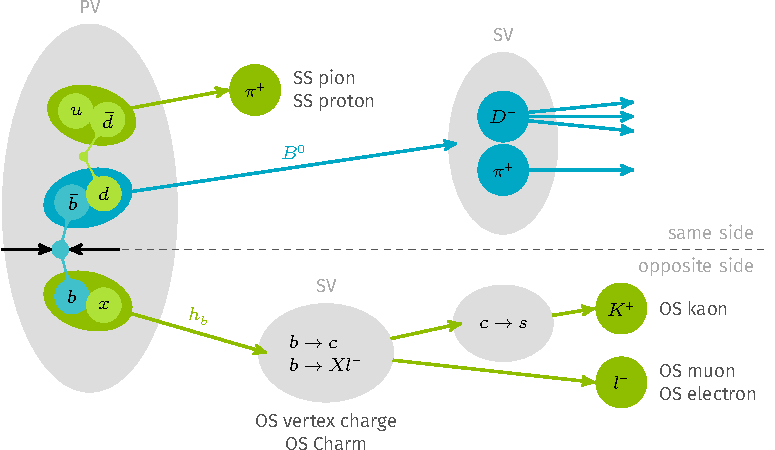
\includegraphics[width=0.8\textwidth]{08FlavourTagging/figs/FTscheme.pdf}
    \caption{Schematic overview of all available \Bz tagging algorithms.}
    \label{fig:taggingalgorithms}
\end{figure}
They can be separated into so-called opposite side (OS) and same side (SS) algorithms.

The OS algorithms exploit the production and decay of the second \bquark-quark which is produced in the proton-proton collision.
By partially reconstructing single decay products as electrons, muons, kaons and \D-mesons associated with the decay of the opposite side \bquark-hadron the initial flavour is inferred.
Furthermore, charged tracks which originate from a secondary vertex, which is displaced from the \ac{PV}, are used to make a decision on the production flavour of the signal $B$-meson.
As the hadronisation and the decay of the OS \bquark-hadron is independent of the signal \B-meson these algorithms can be used for both \Bz and \Bs mesons. Based on \cite{LHCb-PAPER-2011-027, LHCb-PAPER-2015-027} the OS algorithms are briefly described below:
\begin{itemize}
	\item The OS muon and OS electron tagger use the charge of muons and electrons from semileptonic $\bquark\!\to Xl^-$ decays to take a decision on the initial $B$-flavour.
	The charged leptons are selected using a simple cut-based selection.
	To suppress contributions from $\bquark\!\to\cquark\!\to l^+$ decays, which would give the wrong tag decision, for example the transverse momentum of the muon (electron) is required to be larger than \SI[per-mode=symbol]{1.2}{\GeVc} (\SI[per-mode=symbol]{1.0}{\GeVc}).
	Electrons have additionally to satisfy criteria on electron identification variables such as the ratio $\nicefrac{E}{p}>0.8$.
	Here $E$ denotes the energy deposited in the ECAL and $p$ the electron momentum.
	If more than one muon or electron per event survives the selection, the lepton with the highest transverse momentum is chosen to define the flavour of the signal $B$.
	The mistag is estimated with an artificial neural network, which takes as inputs event properties as the number of \ac{PV}s and tracks in the event, $B$-properties as the transverse momentum and various geometrical and kinematic properties of the tagging lepton.
	\item The OS kaon tagger explores the charge of kaons produced in the decay chain $\bquark\!\to\cquark\!\to\squark$.
	Very similar to the lepton taggers the tagging kaon is selected using rectangular cuts based on kinematic and PID observables.
	In case multiple kaons per event pass this selection, the kaon with the highest transverse momentum is fed into an artificial neural network with similar inputs as for the lepton taggers to calculate the mistag estimate $\eta$.
	\item The OS charm tagger selects \D-mesons produced via $\bquark\!\to\cquark$ decays.
	In case of a charged \D-meson the charge of the meson directly hints at the initial flavour, in case of an uncharged \D-meson the charge of the produced kaon is used to infer the flavour of the signal $B$-meson.
	In contrast to the other single track taggers a \ac{BDT} is used to select the \D-meson and estimate the mistag.
	As the OS charm is the newest development on the OS it was developed to have a small overlap concerning the used tagging particles with the other taggers.
	\item The OS vertex charge tagger is the only algorithm which does not reconstruct single particles, but uses the weighted charge of a \ac{SV} associated with the opposite side \bquark-hadron instead.
	In order to do this, the track pair with the highest probability of originating from the opposite side \bquark-hadron is used to build a vertex.
	Following, particles which are compatible with coming from this two-track vertex but not from the \ac{PV} are added to it.
	Finally all tracks of the final \ac{SV} are weighted with their transverse momentum, \pt, and used to calculate a charge
	\begin{equation}
	Q_{\text{vtx}}=\frac{\sum_{i}p_{\mathrm T}^k(i)Q_i}{\sum_{i}p_{\mathrm T}^k(i)}
	\end{equation}
	where the parameter $k$ is optimised to maximise the performance of the tagging algorithm.
	Based on this charge the initial flavour of the signal $B$-meson is then determined.
\end{itemize}

The SS algorithms use remnants of the hadronisation of the signal \B-meson to infer the initial flavour.
As the companion quark of the \bquark-quark is different for \Bz and \Bs-mesons, different algorithms must be used to deduce the initial flavour of the signal \B.

In case of a \Bz (\bquarkbar\dquark) a free \dquarkbar-quark is produced which can hadronise to a pion or proton.
Additionally, the production mechanisms, \eg via the strong decay of an excited $B^{**+}\!\to B^{(*)0}\pip$ can be exploited~\cite{Aaij:2016rdg}.
The SS pion and SS proton taggers use the charge of these companion particles to infer a tag decision.
They were developed on \BdToDpi decays assuming $\Sf=\Sfbar=0$, \ie the decay \BdToDpi is \CP-conserving.
Therefore a potential bias of the analysis cannot be excluded when using these algorithms and they are retrained on $\Bz\!\to\jpsi\Kstarz$.
The basic strategy is similar to the one in Ref.~\cite{Aaij:2016rdg}:
First, tagging particles from the same region of phase space as the signal \B are selected using requirements on PID, kinematic and geometrical observables.
Then, these particles are all used to train a \ac{BDT}, which further selects the final tagging particle and estimates the mistag.
This means in case multiple particles per event pass the selection, the SS pion and SS proton taggers do not select the particle with highest transverse momentum but for all particles the \ac{BDT} response is calculated and the tagging candidate with the largest \ac{BDT} response is chosen afterwards to infer the initial flavour of the signal \B.

On the other hand the hadronisation of a \Bs (\bquarkbar\squark) leads to a \squarkbar-quark which can hadronise to a kaon~\cite{Aaij:2016psi}.
The SS kaon tagger was developed to identify such kaons and works similar for kaons as the SS pion tagger for pions produced in \Bz events.
Since this analysis covers decays of neutral \Bz mesons and the SS kaon tagger is not used, this algorithm is not discussed any further.

\subsection{Performance characteristics}

The predictions of the flavour tagging algorithms are not perfect.
Of $N$ reconstructed candidates only $N'$ candidates get a tag $d$ and mistag $\eta$ assigned, while $N_{\text{U}}$ are untagged.
The $N'$ candidates can be further divided into $N_{\text{W}}$ candidates which are wrongly tagged and $N_{\text{R}}$ correctly tagged candidates.
These imperfections can be reflected by a tagging efficiency
\begin{equation}
\varepsilon_{\text{tag}}=\frac{N_{\text{R}}+N_{\text{W}}}{N_{\text{R}}+N_{\text{W}}+N_{\text{R}}+N_{\text{U}}}\label{eq:tageff}
\end{equation}
and a mistag probability
\begin{equation}
\omega=\frac{N_{\text{W}}}{N_{\text{R}}+N_{\text{W}}}\,.\label{eq:mistag}
\end{equation}
Therefore, in an analysis using flavour tagging to infer the initial \B flavour the number $N_{\Bz}(t)$ ($N_{\Bzb}(t)$) of measured initial \Bz (\Bzb) candidates are
\begin{equation}
\begin{aligned}
N_{\Bz}(t)&=(1-\omega)N_{\Bz}^{\text{true}}(t)+\omega N_{\Bzb}^{\text{true}}(t)\,,\\
N_{\Bzb}(t)&=\omega N_{\Bz}^{\text{true}}(t)+(1-\omega)N_{\Bzb}^{\text{true}}(t)
\end{aligned}
\end{equation}
where $N_{\B}^{\text{true}}$ denotes the true number of initial \Bz and \Bzb candidates.
These quantities need to be transferred further into measurements of \CP-asymmetries such as
\begin{equation}
A_{\CP}(t)=\frac{N_{\Bz}^{\text{true}}(t)-N_{\Bzb}^{\text{true}}(t)}{N_{\Bz}^{\text{true}}(t)+N_{\Bzb}^{\text{true}}(t)}\,.
\end{equation}
For a measured asymmetry the true numbers of initial \Bz- and \Bzb-mesons need to be replaced with the observed yields which leads to
\begin{equation}
A_{\CP}^{\text{meas}}(t)=\frac{N_{\Bz}(t)-N_{\Bzb}(t)}{N_{\Bz}(t)+N_{\Bzb}(t)}=(1-2\omega)A_{\CP}^{\text{theo}}(t)
\end{equation}
with the dilution $D=1-2\omega$.
However, experimentally not only the dilution affects the measured asymmetry but also intrinsic asymmetries $I$ like an asymmetric production of \Bz- and \Bzb-mesons might influence a measurement so that the measured asymmetry can be expressed as
\begin{equation}
A_{\CP}^{\text{meas}}(t)=DA_{\CP}(t)+I\,.
\end{equation}
As the mistag probability is defined in the range $[0, 0.5]$ the dilution can take values between \num{0} and \num{1}.
A large dilution factor is equivalent to a vanishing mistag and hence leads to a larger experimental sensitivity as will be shown below.
To simplify the following discussion the intrinsic asymmetries and dilution are assumed to be time-independent, even if that is not generally valid.
The theoretical asymmetry can then be expressed as
\begin{equation}
A_{\CP}(t)=\frac{1}{D}\left(A_{\CP}^{\text{meas}}(t)-I\right)\,.
\end{equation}
Assuming that all quantities are uncorrelated and gaussian distributed the uncertainty on the theoretical asymmetry is given by
\begin{equation}
\begin{aligned}
\sigma_{A_{\CP}}^2&=\left(\frac{\partial A_{\CP}}{\partial N_{\Bz}}\right)^2\sigma_{N_{\Bz}}^2+\left(\frac{\partial A_{\CP}}{\partial N_{\Bzb}}\right)^2\sigma_{N_{\Bzb}}^2+\left(\frac{\partial A_{\CP}}{\partial I}\right)^2\sigma_{I}^2+\left(\frac{\partial A_{\CP}}{\partial D}\right)^2\sigma_{D}^2\\
&=\frac{1}{D^2}\frac{1}{N_{\Bz}(t)+N_{\Bzb}(t)}\left(1-A_{\CP}^{\text{meas}}(t)\right)+\frac{\sigma_{I}^2}{D^2}+\frac{A_{\CP}^2(t)}{D^2}\sigma_{D}^2\,.
\end{aligned}
\end{equation}
Neglecting the uncertainties on the intrinsic asymmetries and dilution factor and further assuming that the measured asymmetries are small, this expression can be reduced to
\begin{equation}
\sigma_{A_{\CP}}^2=\frac{1}{D^2}\frac{1}{N_{\Bz}(t)+N_{\Bzb}(t)}\,.
\end{equation}
Here it is useful to identify the number of measured \Bz- and \Bzb-candidates as
\begin{equation}
N_{\Bz}(t)+N_{\Bzb}(t)=\varepsilon(t)N
\end{equation}
where $\varepsilon$ includes all efficiencies either in the trigger, reconstruction, selection or the flavour tagging.
Regarding the flavour tagging this means that the uncertainty on a \CP-asymmetry is given by
\begin{equation}
\sigma_{A_{\CP}}=\frac{1}{\sqrt{\varepsilon_{\text{tag}}D^2N}}=\frac{1}{\sqrt{\varepsilon_{\text{eff}}N}}
\end{equation}
where the effective tagging efficiency $\varepsilon_{\text{eff}}=\varepsilon_{\text{tag}}D^2$ was introduced.
As one can see, this efficiency defines the experimental sensitivity of the measurement as it effectively reduces the number of candidates.
It also becomes obvious that the tagging efficiency introduced in \cref{eq:tageff} and the mistag probability defined in \cref{eq:mistag} are not individually suitable for determining the performance of different tagging algorithms.
Instead the tagging efficiency, which is also denoted as tagging power, must be used.

Rather than using an average mistag $\omega$ the mistag estimate $\eta$ of the various tagging algorithms can be used.
To do this, the estimated mistag has to be calibrated with a calibration function $\omega(\eta)$ (more details on the calibration are given in \cref{sec:CombAndCalib}), what gives a per-event tagging power, defined as
\begin{equation}
\varepsilon_{\text{eff}}=\frac{1}{N}\sum_{i=1}^{N}D_i^2=\frac{1}{N}\sum_{i=1}^{N}\left(1-2\omega(\eta_i)\right)^2\,.
\end{equation}
Here the sum is iterating over all candidates and for untagged candidates the mistag probability is defined to be \num{0.5} ($D_i=0$).

When considering only tagged candidates, the effective tagging efficiency reduces to a pseudo tagging power, which is effectively the same as average of the dilution squared in the respective sample:
\begin{equation}
\left<D^2\right>=\frac{1}{N_{\text{R}}+N_{\text{W}}}\sum_{i=1}^{N_{\text{R}}+N_{\text{W}}}\left(1-2\omega(\eta_i)\right)^2\,.
\end{equation}

\subsection{Combination and calibration of flavour tagging algorithms}
\label{sec:CombAndCalib}

To improve the overall performance of the flavour tagging the individual algorithms are combined to form one single tag decision and mistag for the OS ($d_{\text{OS}}$ and $\eta_{\text{OS}}$) and a tag decision and mistag for the SS ($d_{\text{SS}}$ and $\eta_{\text{SS}}$).
This is done by calculating the combined probability, that a \B-candidate contains a \bquark-quark
\begin{equation}
P(\bquark)=\frac{p(\bquark)}{p(\bquark)+p(\bquarkbar)}\hspace{0.5cm}\text{and}\hspace{0.5cm}P(\bquarkbar)=1-P(\bquark)\,.
\end{equation}
The probabilities $p(\bquark)$ and $p(\bquarkbar)$ are defined as
\begin{equation}
p(\bquark)=\prod_{i}\left(\frac{1+d_i}{2}-d_i\left(1-\eta_i\right)\right)
\end{equation}
and
\begin{equation}
p(\bquarkbar)=\prod_{i}\left(\frac{1-d_i}{2}+d_i\left(1-\eta_i\right)\right)
\end{equation}
where $d_i$ ($\eta_i$) are the tag decisions (mistag estimates) of the individual tagging algorithms.
The combined tag decision and mistag are now defined as $d=-1$ and $\eta=1-P(\bquark)$ if $P(\bquark)>P(\bquarkbar)$ and as $d=+1$ and $\eta=P(\bquark)$ if $P(\bquark)<P(\bquarkbar)$.

As mentioned before, the output of the flavour tagging algorithms is mostly the result of multivariate classifiers, which are trained on flavour specific \B decays.
This output is then transformed into a mistag estimate $\eta$ and crosschecked on another flavour specific validation sample.
However, the training and validation sample are usually different from the signal decay used in a \CP-violation measurement.
This differences are caused by different trigger and selection criteria and can influence the distributions which are used by the multivariate classifier to estimate the mistag.
Consequently, the mistag must be calibrated on a dedicated flavour specific decay, which shows at best kinematically similar distributions compared to the signal decay.
For the OS taggers this is most often done using charged decay modes, as the charge of the final state particles allows to directly infer the production flavour.
Instead, to calibrate the SS taggers a decay mode with the same initial \B flavour is needed, as these taggers highly depend on the hadronisation process.
In this analysis the OS taggers are calibrated using $\Bu\!\to\Dz\pip$, where the bachelor pion allows to infer the initial flavour, while the SS taggers are calibrated using $\Bz\!\to\jpsi\Kstarz$.

So far, for all analyses at \lhcb a linear calibration function of the form
\begin{equation}
\omega(\eta)=\tilde{p}_0+\tilde{p}_1\left(\eta-\left<\eta\right>\right)\label{eq:linCalib}
\end{equation}
where the arithmetic mean $\left<\eta\right>$ of the estimated mistag is used to decorrelate the calibration parameters $p_0$ and $p_1$, was sufficient.
Using this calibration function a perfect calibration, \ie $\omega=\eta$, would result in $\tilde{p}_0=\left<\eta\right>$ and $\tilde{p}_1=1$.
Yet, the performance of the tagger can depend on the initial \B flavour:
If the interaction rates of charged decay products (\eg the kaons used by the OS kaon tagger) with the detector material depend on the charge, the mistags will also depend on the flavour of the initial \B meson.
Such asymmetry yields in an additional dilution factor, which needs to be understood and properly described.
This can be achieved by using different calibration functions for \Bz- and \Bzb-mesons.
In the simple linear case these calibration functions are
\begin{equation}
\begin{aligned}
\omega&=p_0+p_1+\left(\eta-\left<\eta\right>\right)\,,\\
\overline{\omega}&=\overline{p}_0+\overline{p}_1+\left(\eta-\left<\eta\right>\right)\,.
\end{aligned}
\end{equation}
These different calibration parameters are furthermore linked to each other via the average calibration parameters $\tilde{p}_i$ used in \cref{eq:linCalib} and corresponding differences $\Delta p_i$ defined as
\begin{equation}
\tilde{p}_i=\frac{p_i+\overline{p}_i}{2}\hspace{0.5cm}\text{and}\hspace{0.5cm}\Delta p_i=p_i-\overline{p}_i\,\,.
\end{equation}

However, due to the large number of \BdToDpi signal candidates small effects that were hidden in the statistical uncertainties before become significant.
Therefore more sophisticated calibration functions are needed to calibrate the flavour tagging algorithms.
The adopted models are called generalised linear models (GLM)~\cite{GLM} and have the following form:
\begin{equation}
\WorWbar(\eta) = g\left(h(\eta)\right) = g\left( g^{-1} (\eta) + \sum_{i=1}^{N} \left(\tilde{p}_i \kern 0.0em\optbar{\kern -0.0em +} \frac{\Delta p_i}{2}\right) f_i(\eta)\right)\,.
\end{equation}
The functions $f_i$ are the so-called \emph{basis functions}, which for example can be simple poynomials or natural spline functions~\cite{Nsplines}.
To minimise the correlation between the $\tilde{p}_i$ and $\Delta p_i$ parameters the \emph{basis functions} are orthogonalised using the Gram-Schmidt method~\cite{GramSchmidt}.
The function $g$ is referred to as \emph{link function}, which is usually defined as the inverse cumulative distribution function, to map all input values to the range $[0,1]$, \ie an interval which can be interpreted as a probability.
As the mistag is only defined in the range $[0, 0.5]$ it is possible, that after applying a calibration function with this \emph{link function} the mistag is larger than \num{0.5}.
In this case an arbitrary decision has to be taken how such candidates are further treated.
Possible options are to either flip the corresponding tag decision $d\to-d$ and adjust the mistag $\omega\to1-\omega$ or to mark the candidate as untagged with a mistag of \num{0.5}.
The latter possibility leads to fit instabilities in the decay-time fit when the calibration parameters are not fixed, but allowed to float or constrained by means of a Gaussian function.
This is due to the fact that for a floating or constrained calibration the ratio of tagged and untagged candidates varies during the minimisation and the changes to the likelihood are not continous.
On the other hand, a flip of the tagdesicion may yield in a bias of the \CP-parameters as shown in \cref{sec:ValLinkFunction}.
Therefore, the modified logistic function
\begin{equation}
g(h)=\frac{1}{2\left(1+e^h\right)}\label{eq:modlink}
\end{equation}
is used as \emph{link function}, which maps all input values into the range $[0, 0.5]$ and hence assures that all calibrated mistags are well defined.

To not rely on possible binning effects on the estimated mistag $\eta$ or the mistag probability $\omega$, the calibration functions are determined using an unbinned maximum-likelihood method, the so-called binomial regression~\cite{BinRegression}.

\section{Flavour tagging strategy}
\label{sec:taggingstrategy}

In this analysis the combination of all available OS algorithms is used, while for the SS both taggers designed to infer the initial flavour of \Bz-mesons are combined into one single tag decision and mistag.
The OS taggers were all developed and trained on a datasample of $\Bu\!\to\jpsi\Kp$ decays, except for the OS charm tagger, whose BDT was trained on a mixed sample of simulated $\Bu\!\to\jpsi\Kp$, $\Bz\!\to\jpsi\Kstarz$ and $\Bs\!\to\jpsi\phi$ decays.
As the OS taggers are independent of the initial signal \B they can be used in this default version.
As control channel the decay $\Bu\!\to\Dz\pip$ is used.
As mentioned before, the SS pion and the SS proton taggers were deveolped and trained on a datasample of \BdToDpi decays, assuming no \CP-violation.
The use of these algorithms could therefore bias the measurement of \Sf and \Sfbar and hence both taggers are retrained (more details given in \cref{sec:retrainSSpion} and \cref{sec:retrainSSproton}).

To include the flavour tagging in the decay rates given in \crefrange{eq:DecRateB2Dmpip}{eq:DecRateBb2Dppim} the expressions for the \CP-parameters \Sf and \Cf need to be extended to
\begin{equation}
\begin{aligned}
\Sf&\to\left(\Delta^--\Delta^+\right)\Sf\,\,,\\
\Cf&\to\left(\Delta^--\Delta^+\right)\Cf\,\,.\label{eq:decRateCorrectFT}
\end{aligned}
\end{equation}
Similar equations hold also for \Sfbar and \Cfbar.
The coefficients $\Delta^\pm$ contain the calibration functions and tagging efficiencies $\varepsilon_{\text{tag}}^{\text{OS}}$ and $\varepsilon_{\text{tag}}^{\text{SS}}$.
They are defined as
\begin{align}
\Delta^\pm&=\frac{1}{2}\varepsilon_{\text{\tiny tag}}^{\text{\tiny OS}}\left[1-\varepsilon_{\text{\tiny tag}}^{\text{\tiny SS}}+d^{\text{\tiny OS}}\left(1-\varepsilon_{\text{\tiny tag}}^{\text{\tiny SS}}-2\omega(\eta^{\text{\tiny OS}})\left(1+\varepsilon_{\text{\tiny tag}}^{\text{\tiny SS}}\right)\right)\right]\nonumber\\
&\pm\frac{1}{2}\varepsilon_{\text{\tiny tag}}^{\text{\tiny OS}}\left[1-\varepsilon_{\text{\tiny tag}}^{\text{\tiny SS}}+d^{\text{\tiny OS}}\left(1-\varepsilon_{\text{\tiny tag}}^{\text{\tiny SS}}-2\overline{\omega}(\eta^{\text{\tiny OS}})\left(1+\varepsilon_{\text{\tiny tag}}^{\text{\tiny SS}}\right)\right)\right]
\end{align}
for candidates which are only tagged by the OS tagger combination.
To obtain the expression for candidates only tagged by the SS taggers, all superscripts need to be exchanged with $\text{OS}\leftrightarrow\text{SS}$.
For candidates which are tagged by both, the OS tagger combination and the SS taggers the coefficients can be written as
\begin{align}
\Delta^\pm&=\frac{1}{4}\varepsilon_{\text{\tiny tag}}^{\text{\tiny OS}}\varepsilon_{\text{\tiny tag}}^{\text{\tiny SS}}\left[1+\hspace{-3mm}\sum_{j=\text{\tiny OS, SS}}\hspace{-2mm}d_j\left(1-2\omega(\eta_j)\right)+d^{\text{\tiny OS}}d^{\text{\tiny SS}}\left(1-2\omega(\eta_j)+2\omega(\eta^{\text{\tiny OS}})\omega(\eta^{\text{\tiny SS}})\right)\right]\nonumber\\
&\pm\frac{1}{4}\varepsilon_{\text{\tiny tag}}^{\text{\tiny OS}}\varepsilon_{\text{\tiny tag}}^{\text{\tiny SS}}\left[1+\hspace{-3mm}\sum_{j=\text{\tiny OS, SS}}\hspace{-2mm}d_j\left(1-2\overline{\omega}(\eta_j)\right)+d^{\text{\tiny OS}}d^{\text{\tiny SS}}\left(1-2\overline{\omega}(\eta_j)+2\overline{\omega}(\eta^{\text{\tiny OS}})\overline{\omega}(\eta^{\text{\tiny SS}})\right)\right]\,.
\end{align}

The flavour specific control samples ($\Bu\!\to\Dz\pip$ for the OS, $\Bz\!\to\jpsi\Kstarz$ for the SS) are used to determine the functional form of the calibration function $\omega(\eta)$.
Unlike other flavour tagged analyses at \lhcb the calibration parameters can be determined directly in the decay-time fit as floating nuisance parameter of the likelihood function in \BdToDpi.
This is possible because the parameters \Cf and \Cfbar are fixed to \num{1} and \num{-1} as the ratio $r$ (see \cref{eq:ratioDpi}) is expected to be too small to allow a significant measurement of both parameters.
As a result, the cosine term allows to determine the calibration parameters independently of the sine term.
A qualitative explanation of this is given in \cref{fig:FTstrategy}.
\begin{figure}[tbp]
    \centering
    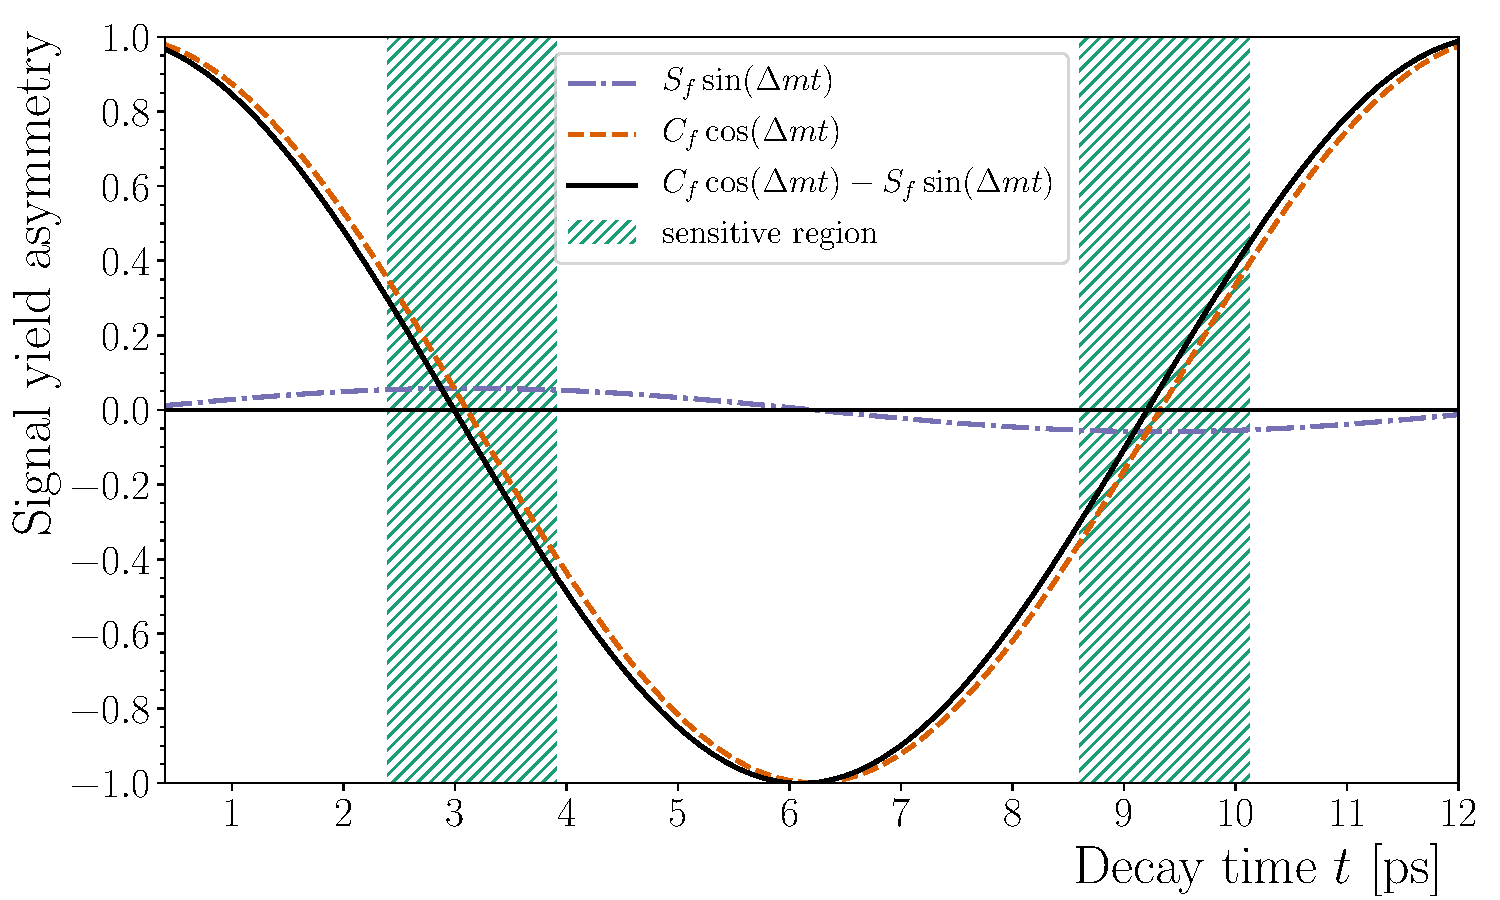
\includegraphics[width=0.48\textwidth]{08FlavourTagging/figs/oscillation_f.pdf}
    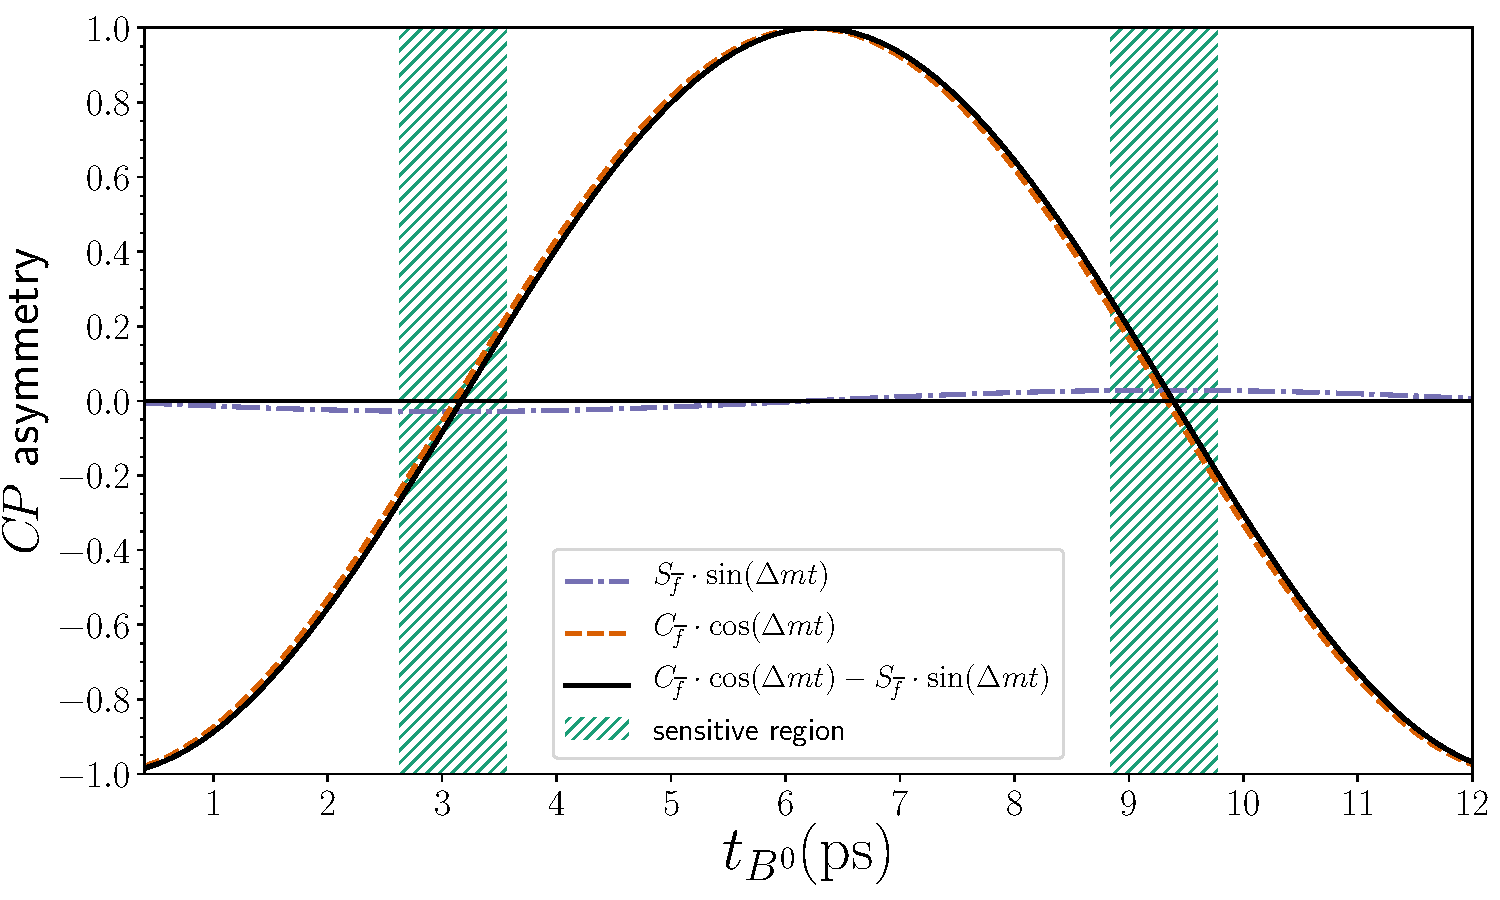
\includegraphics[width=0.48\textwidth]{08FlavourTagging/figs/oscillation_fbar.pdf}
    \caption{Time-dependent asymmetries for \Bzb versus \Bz for the \Dm\pip (left) and \Dp\pim (right) final states.
    The values for the \CP parameters are taken from simulation and no experimental dilutions are included.
    Since the deviation of the sum of both trigonometric functions from a single cosine function is very small due to the tiny values of \Sf and \Sfbar, the maximum sensitivity is achieved in the regions of the zero-points, \ie where the amplitude of $\cos(\dm t)$ and $\sin(\dm t)$ are of similar size.
    These regions are denoted as \enquote{sensitive regions} in both plots.
    In the \enquote{non-sensitive regions}, where the cosine-function is completely dominating, additional diluting effects due to the tagging calibration can be determined.}
    \label{fig:FTstrategy}
\end{figure}

When determining all calibration parameters directly in the signal sample no assumptions for the portability of the calibration from a control channel is needed.
This portability in principle can be limited due to kinematic differences between the control sample and the signal sample leading to different flavour tagging calibrations.
It is probed using simulated events of both, the control sample and the signal sample.
When checking the portability of the calibrations from $\Bu\!\to\Dz\pip$ and $\Bz\!\to\jpsi\Kstarz$ to \BdToDpi a bias on \Sf and \Sfbar of roughly the size of their statistical uncertainty arises.
This bias can be reduced when floating the calibration parameters (more details on this are given in \cref{sec:decTimeFitVal}).
Furthermore, the precision of the calibration parameters for the SS tagger combination obtained in the decay-time fit to \mbox{\BdToDpi} is much smaller compared to the precision on the control channel, while for the OS tagger combination the uncertainty on the signal sample increases only slightly compared to the uncertainty obtained on the control sample.
However, determining the calibration parameters in the final decay-time fit leads to an increased statistical uncertainty on the \CP-parameters \Sf and \Sfbar due to the additional degrees of freedom in the fit.
This is compensated by the fact that the systematic uncertainty for the portability of the calibration, which is often the largest systematic uncertainty for flavour tagged analyses at \lhcb, is not needed.

A quantitative validation of this strategy was done by a collaborator on pseudoexperiments:
Generating pseudoexperiments and floating the parameters \Cf and \Cfbar in the fit showed a non-negligible bias for the parameters \Sf and \Sfbar, while fixing the coefficients \Cf and \Cfbar in the fit showed unbiased results on all fitted parameters.
Therefore this strategy is adopted for the extraction of the calibration parameters.
Finally it should be noted here that possible deviations from the assumption of $\Cf=-\Cfbar=1$ are taken into account in the systematic uncertainties (\cref{ch:systeamticUncerts}).

Thus, the studies presented in the following sections do not aim to obtain the calibration parameters.
Instead, on the one hand, they are used to determine the functional form of the calibration function, which is used in the decay-time fit described in \cref{sec:ExtractCPobs}.
On the other hand, the obtained parameter values of the calibration function can be used as reference values for the decay-time fit, as even if they are not expected to agree perfectly, both parameter sets should be in the same interval.

\section{Same side tagging calibration}
\label{sec:SScalibration}

The SS tagger combination is retrained and calibrated on the datasample of $\Bz\!\to\jpsi\Kstarz$ candidates corresponding to \SI{3}{\per\femto\barn}, recorded in \num{2011} and \num{2012} at centre-of-mass energies of \SI{7}{\tera\electronvolt} and \SI{8}{\tera\electronvolt}, respectively.
It is used because $\Bz\!\to\jpsi\Kstarz$ is the only flavour-specific decay mode of \Bz-mesons with a sufficient large statistic beside the signal mode of \BdToDpi at \lhcb.
The strategy follows mainly the one which was used to train the original taggers on \BdToDpi what is described in Ref.~\cite{Aaij:2016rdg}.
Only one additional step is implemented:
The distributions of $\Bz\!\to\jpsi\Kstarz$ candidates are kinematically weighted to match the distributions of \BdToDpi candidates.
The general procedure is quite similar for both tagging algorithms and looks as following:
\begin{itemize}
	\item The $\Bz\!\to\jpsi\Kstarz$ sample is selected and a fit to the invariant mass is performed, in order to separate the signal and background components statistically.
	Using the \emph{sPlot} method weights are calculated, which allow to obtain the signal-component distributions of other variables. This is reported in \cref{sec:PrepBd2JpsiKstSample}
	\item The distributions of transverse momentum \pt, pseudo-rapidity $\eta'$ and azimuthal angle $\phi$ of the \Bz candidate, the number of tracks and the number of \ac{PV}s in the event and a distribution of Hlt2 trigger decisions for $\Bz\!\to\jpsi\Kstarz$ candidates are weighted to match those of the \BdToDpi candidates.
	This has two reasons: First the performance of the BDT is potentially improved when applying to \BdToDpi, second the portability of the functional form of the calibration is assured, and calibration parameters obtained can be better used as reference values.
	\item The tagging particles, whose charge is correlated with the initial \B flavour are selected
	\item Finally the datasample is divided into three subsamples:
	\begin{itemize}
		\item The first third of the sample is used to train a BDT to separate correctly and wrongly charged tagging particles.
		Hereby correctly tagged means that the charge of the tagging particle would indicate the correct tag, while wrongly tagged denotes exactly the opposite situation: The tagging particles' charge would indicate the wrong tag decision.
		To reduce the number of oscillated \Bz-mesons only \Bz-mesons with a decay time smaller than the first maximum of the oscillation are used.
		Therefore, following the procedure in Ref.~\cite{Aaij:2016rdg}, \Bz-mesons used in the training are required to have a a decay time smaller than \SI{2.2}{\pico\second}.
		\item On the second subsample the BDT is tested in order to avoid effects as overtraining.
		Furthermore, both, the first training sample and this second testing sample are used to determine the mistag as a function of the BDT response. For this latter step the requirement on the \Bz decay time is removed, as a full time-dependent analysis of the \Bz oscillation is performed.
		\item Finally on the last third the SS taggers are combined and the functional form of the calibration is determined together with reference values for the calibration parameters obtained in the decay-time fit described in \cref{sec:ExtractCPobs}.
	\end{itemize}
\end{itemize}

\subsection[head={Preparation of the $\Bz\!\to\jpsi\Kstarz$ samples},tocentry={Preparation of the $\Bz\!\to\jpsi\Kstarz$ samples}]{Preparation of the $\symbfsf{\Bz\!\to\jpsi\Kstarz}$ samples}
\label{sec:PrepBd2JpsiKstSample}


The decay $\Bz\!\to\jpsi\Kstarz$ is reconstructed using the decays $\jpsi\!\to\mup\mun$ and \mbox{$\Kstarz\!\to\Kp\pim$}.
The cuts applied in the stripping are listed in \cref{tab:JpsiKstStripping}.
Again, to achieve  better compatibility between $\Bz\!\to\jpsi\Kstarz$ and the signal decay \BdToDpi, the same trigger requirements as for the signal mode are applied.
After the trigger requirements the \Kstarz- and the \jpsi-meson are requried to fulfill the cuts shown in \cref{tab:selJpsiKst}.
\begin{table}[tbp]
	\centering
	\caption{Stripping cuts for the decay $\Bz\!\to\jpsi\Kstarz$ with $\jpsi\!\to\mup\mun$ and $\Kstarz\!\to\Kp\pim$.
	For the charged tracks the more stringent requirements for the bachelor track are given in brackets.
	For the impact parameter the shortcut IP is used, DOCA denotes the distance of closest approach of the respective \Kstarz or \jpsi mesons and $m_{p^+p^-}$ denotes the invariant mass of the \mup\mun or \Kp\pim combination.}
	\begin{tabular}{ccc}
		\toprule
		\multicolumn{3}{c}{\muon requirements}\\
		\midrule
		transverse momentum \pt 	& \multicolumn{2}{c}{$>\SI[per-mode=symbol]{500}{\MeVc}$} \\
		\dllmupi					& \multicolumn{2}{c}{$>0.0$} \\
		\midrule
		resonances-requirements & \jpsi & \Kstarz\\
		\midrule
		transverse momentum \pt 							& - 								& $>\SI[per-mode=symbol]{500}{\MeVc}$ \\
		DOCA $\chi^2$										& $<20.0$ 							& $<30.0$ \\
		$\left|m_{p^+p^-}-m_{\jpsi}^{\text{PDG}}\right|$	& \SI[per-mode=symbol]{150}{\MeVcc} & \SI[per-mode=symbol]{300}{\MeVcc} \\
		decay vertex $\chi^2$ 								& $<16.0$ 							& $<25.0$ \\
		\midrule
		\multicolumn{3}{c}{\Bz-meson requirements}\\
		\midrule
		reconstructed decay time $t$ 	& \multicolumn{2}{c}{$>\SI{0.2}{\pico\second}$} \\
		\bottomrule
	\end{tabular}
	\label{tab:JpsiKstStripping}
\end{table}
\begin{table}[tbp]
	\centering
	\caption{Cuts to select $\Bz\!\to\jpsi\Kstarz$ candidates.
	The transverse momentum is denoted as \pt, for the impact parameter the shortcut IP is used and $h$ denotes a kaon or pion.}
	\begin{tabular}{cc}
		\toprule
		\jpsi/\muon requirements & \Kstarz/(\kaon, \pion) requirements\\
		\midrule
		$\dllmupi>0$																& $\dllkpi>0$ \hspace{0,2cm} for kaons \\
		track $\nicefrac{\chi^2}{\text{ndof}}<4$ 									& track $\nicefrac{\chi^2}{\text{ndof}}<4$ \\
		$\pt(\mup)>\SI{500}{\MeVc}||\pt(\mun)>\SI[per-mode=symbol]{500}{\MeVc}$ 	& $\pt(\Kstarz)>\SI[per-mode=symbol]{1000}{\MeVc}$\\
		vertex $\chi^2$/ndof$<16$ of \jpsi 											& vertex $\chi^2$/ndof$<16$ of \Kstarz\\
		$\left|m_{J/\psi}-m_\text{PDG}\right|<\SI[per-mode=symbol]{80}{\MeVcc}$ 	& $\left|m_{\Kstarz}-m^\text{PDG}\right|<\SI[per-mode=symbol]{70}{\MeVcc}$\\
		\bottomrule
	\end{tabular}
	\label{tab:selJpsiKst}
\end{table}
Additionally only \Bz-candidates with an invariant mass within the range $[5100, 5450]\,$\si[per-mode=symbol]{\MeVcc}, a transverse momentum larger than \SI{1}{\GeVc}, the minimal $\chi^2$ of the impact parameter w.r.t. the \ac{PV} smaller than \num{25} and $\nicefrac{\chi^2}{\text{ndof}}$ of the decay vertex smaller than ten are selected.
Last the DTF $\nicefrac{\chi^2}{\text{ndof}}$ is required to be smaller than five and the number of \ac{PV}s in the event has to be one, or in case an event has more than one \ac{PV} the impact parameter $\chi^2$ has to be larger than \num{50}.
In case of multiple \Bz candidates the one with the smallest DTF $\nicefrac{\chi^2}{\text{ndof}}$ is chosen.

To extract \emph{sWeights} a fit to the invariant \Bz mass, stemming from the DTF with a constraint on the known \jpsi mass is performed.
The signal model consists of a sum of two double-sided Hypatia functions with a shared mean value, the background is parametrised using an exponential function.
The first Hypatia function describes mainly $\Bz\!\to\jpsi\Kstarz$ candidates without photon radiation in the final state, while the second Hypatia shows a large tail towards smaller invariant masses.
The tail parameters $a_i$ and $n_i$ of both Hypatia functions are determined on simulated events.
Moreover the fraction between both signal components and the parameter $\lambda$ of the Hypatia describing the \Bz candidates with harder photon radiation are taken from fits to simulated samples.
All remaining parameters are floating.
The fit which is performed in the range $[5200, 5350]\,$\si[per-mode=symbol]{\MeVcc} is shown in \cref{fig:massFitJpsiKst} and the resulting yields are given in \cref{tab:yieldsJpsiKst}.
\begin{figure}[tbp]
    \centering
    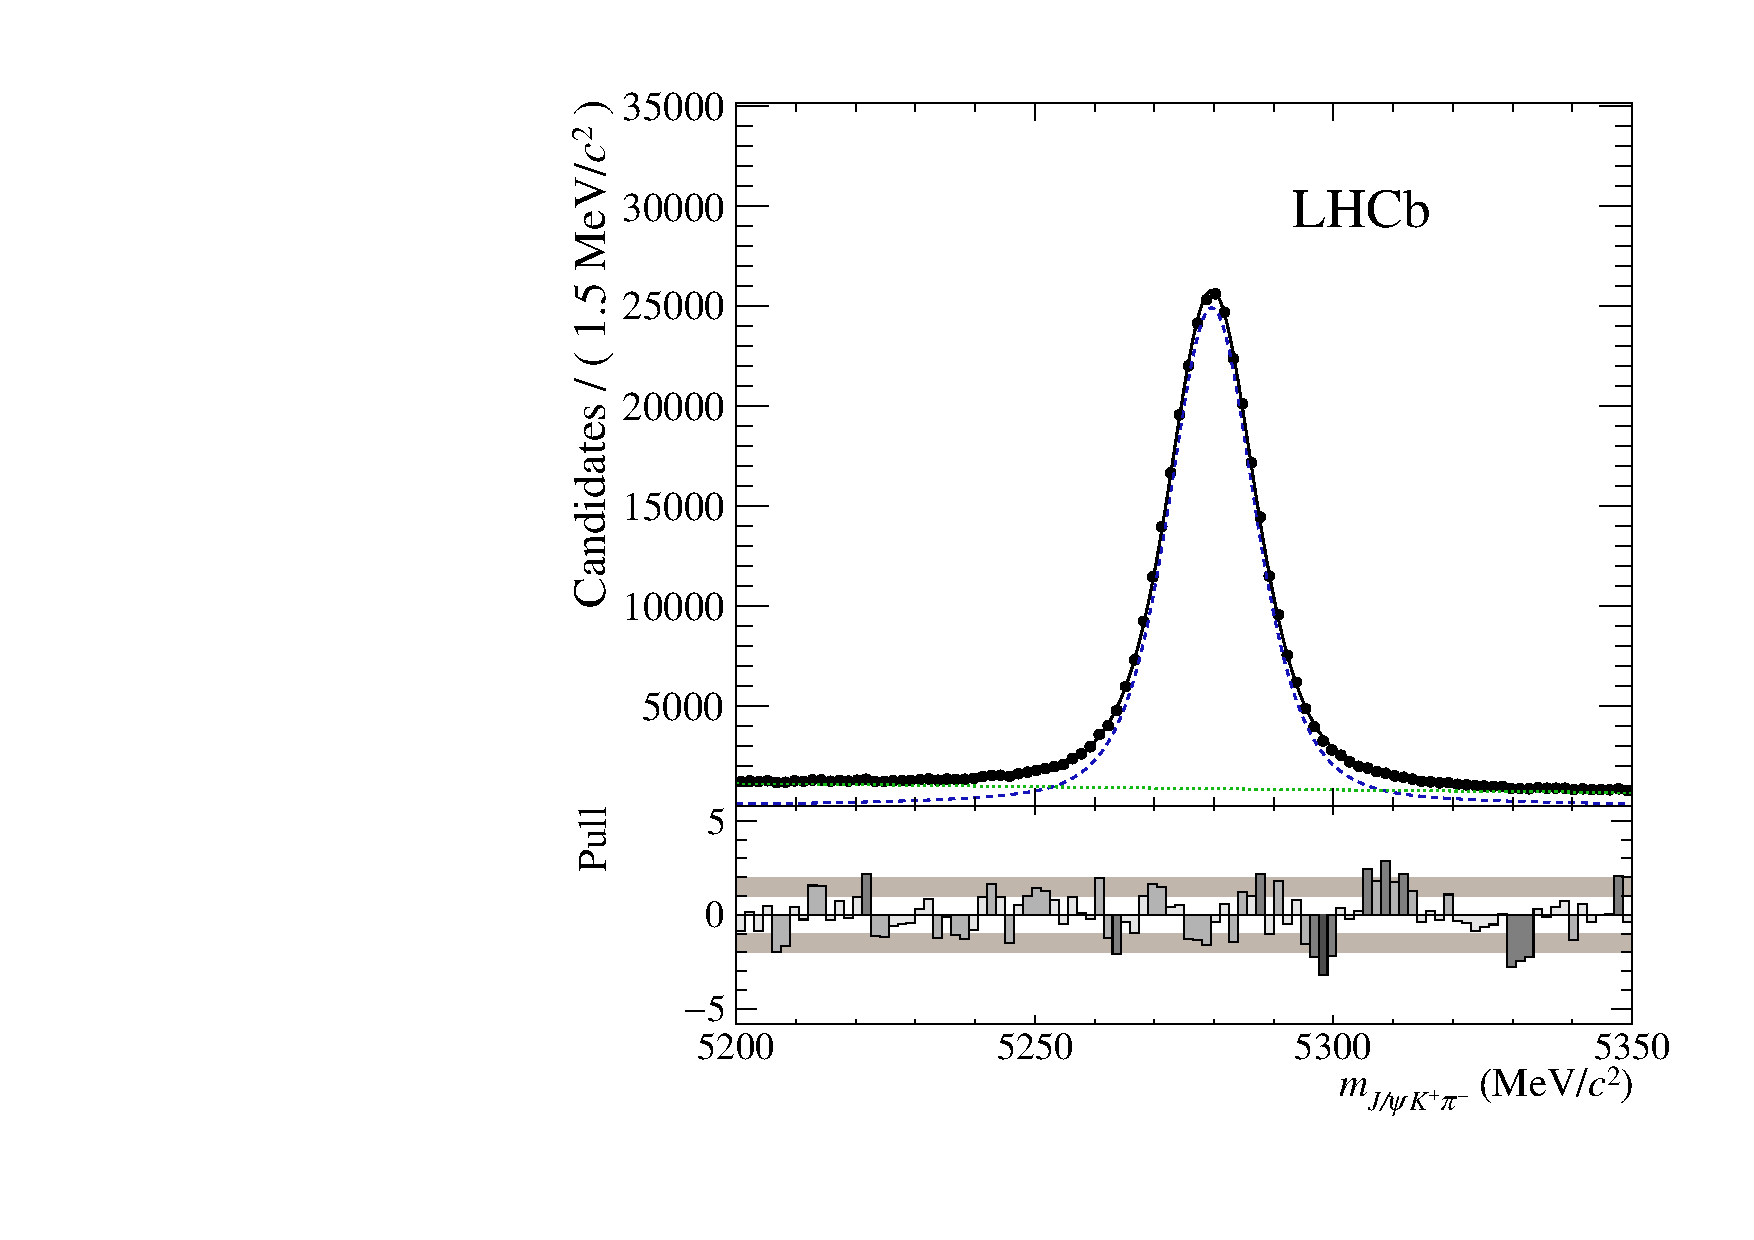
\includegraphics[width=0.5\textwidth]{08FlavourTagging/figs/BmassJpsiKst_pull.pdf}
    \caption{Fit to the invariant mass of the $\Bz\!\to\jpsi\Kstarz$ candidates with a constraint on the known \jpsi mass.
    The data is represented by the black points, the black solid line shows the full PDF, the blue dashed line shows the signal componente and the background component is represented by the dotted yellow line.}
    \label{fig:massFitJpsiKst}
\end{figure}
\begin{table}[tbp]
	\centering
	\caption{Fitted Yields of the $\Bz\!\to\jpsi\Kstarz$ component and the combinatorial background.}
	\begin{tabular}{SS}
		\toprule
		{Parameter} & {Yield} \\
		\midrule
		{$N_{\Bz\!\to\D\pion}^{\pion}$}	& 351507\pm662 \\
		{$N_{\text{bkg}}^{\pion}$}		& 88630\pm419 \\
		\bottomrule
	\end{tabular}
	\label{tab:yieldsJpsiKst}
\end{table}

The last preparation step for the data sample is then to weight certain \emph{sWeighted} distributions of $\Bz\!\to\jpsi\Kstarz$ candidates to match the corresponding distributions of the \BdToDpi candidates.
The observables which are weighted are chosen as they are known to most influence the tagging responses:
These observables are the transverse momentum \pt, the pseudo-rapidity $\eta'$ and the azimuthal angle $\phi$ of the \Bz candidate as well as the number of tracks and the number of \ac{PV}s in the event.
Additionally, an observable containing the composition of the used trigger lines is weighted.
For this observables the categories \num{1}, \num{2} and \num{3} contain candidates which are exclusively triggered TOS by the \verb!Hlt2Topo2BodyBBDTDecision!, \verb!Hlt2Topo3BodyBBDTDecision! or \verb!Hlt2Topo4BodyBBDTDecision! line, respectively.
Category \num{4} contains candidates triggered TOS exclusively by the overlap of the \verb!Hlt2Topo2BodyBBDTDecision! and \verb!Hlt2Topo3BodyBBDTDecision! lines, candidates triggered exculsively TOS by the overlap of the \verb!Hlt2Topo2BodyBBDTDecision! and \verb!Hlt2Topo4BodyBBDTDecision! lines are classified in category \num{5} and candidates triggered exclusively TOS by the overlap of the \verb!Hlt2Topo3BodyBBDTDecision! and \verb!Hlt2Topo4BodyBBDTDecision! lines are in category \num{6}.
The last category (\num{7}) contains candidates which are triggered by all three Hlt2 lines.

Instead of weighting the six-dimensional parameter space using a six-dimensional histogram a BDT based approach is chosen.
In this approach, the parameter space is split in several large regions, which are separated using binary decision trees.
These trees maximise a symmetrised $\chi^2$
\begin{equation}
\chi^2=\sum_{i}\frac{\left(N_{i,\text{source}}-N_{i,\text{target}}\right)^2}{N_{i,\text{source}}+N_{i,\text{target}}}
\end{equation}
where $N_{i,\text{source}}$ are the number of candidates in the $i$th bin of the distribution which should be weighted and $N_{i,\text{target}}$ are the number of candidates in the $i$th bin of the target distribution.
For all leaves of a decision tree a prediction $p$ is calculated following
\begin{equation}
p=\log\frac{N_{i,\text{target}}}{N_{i,\text{source}}}\,,
\end{equation}
what is used to calculate the weights as
\begin{equation}
w=\begin{cases} w, &\, \text{if event from target distribution}\\ we^{p}, &\, \text{if event from source distribution\,\,.} \end{cases}
\end{equation}
These steps are then repeated for each decision tree.
In this case the BDT is built out of \num{40} trees with a maximum depth of three.
Each leave has to contain a minimum number of \num{200} candidates and the boosting method is Gradient boosting~\cite{Friedman00greedyfunction}.
The distributions of the original and weighted $\Bz\!\to\jpsi\Kstarz$ and \BdToDpi candidates is shown in \cref{fig:reweightingSS}.
\begin{figure}[tbp]
    \centering
    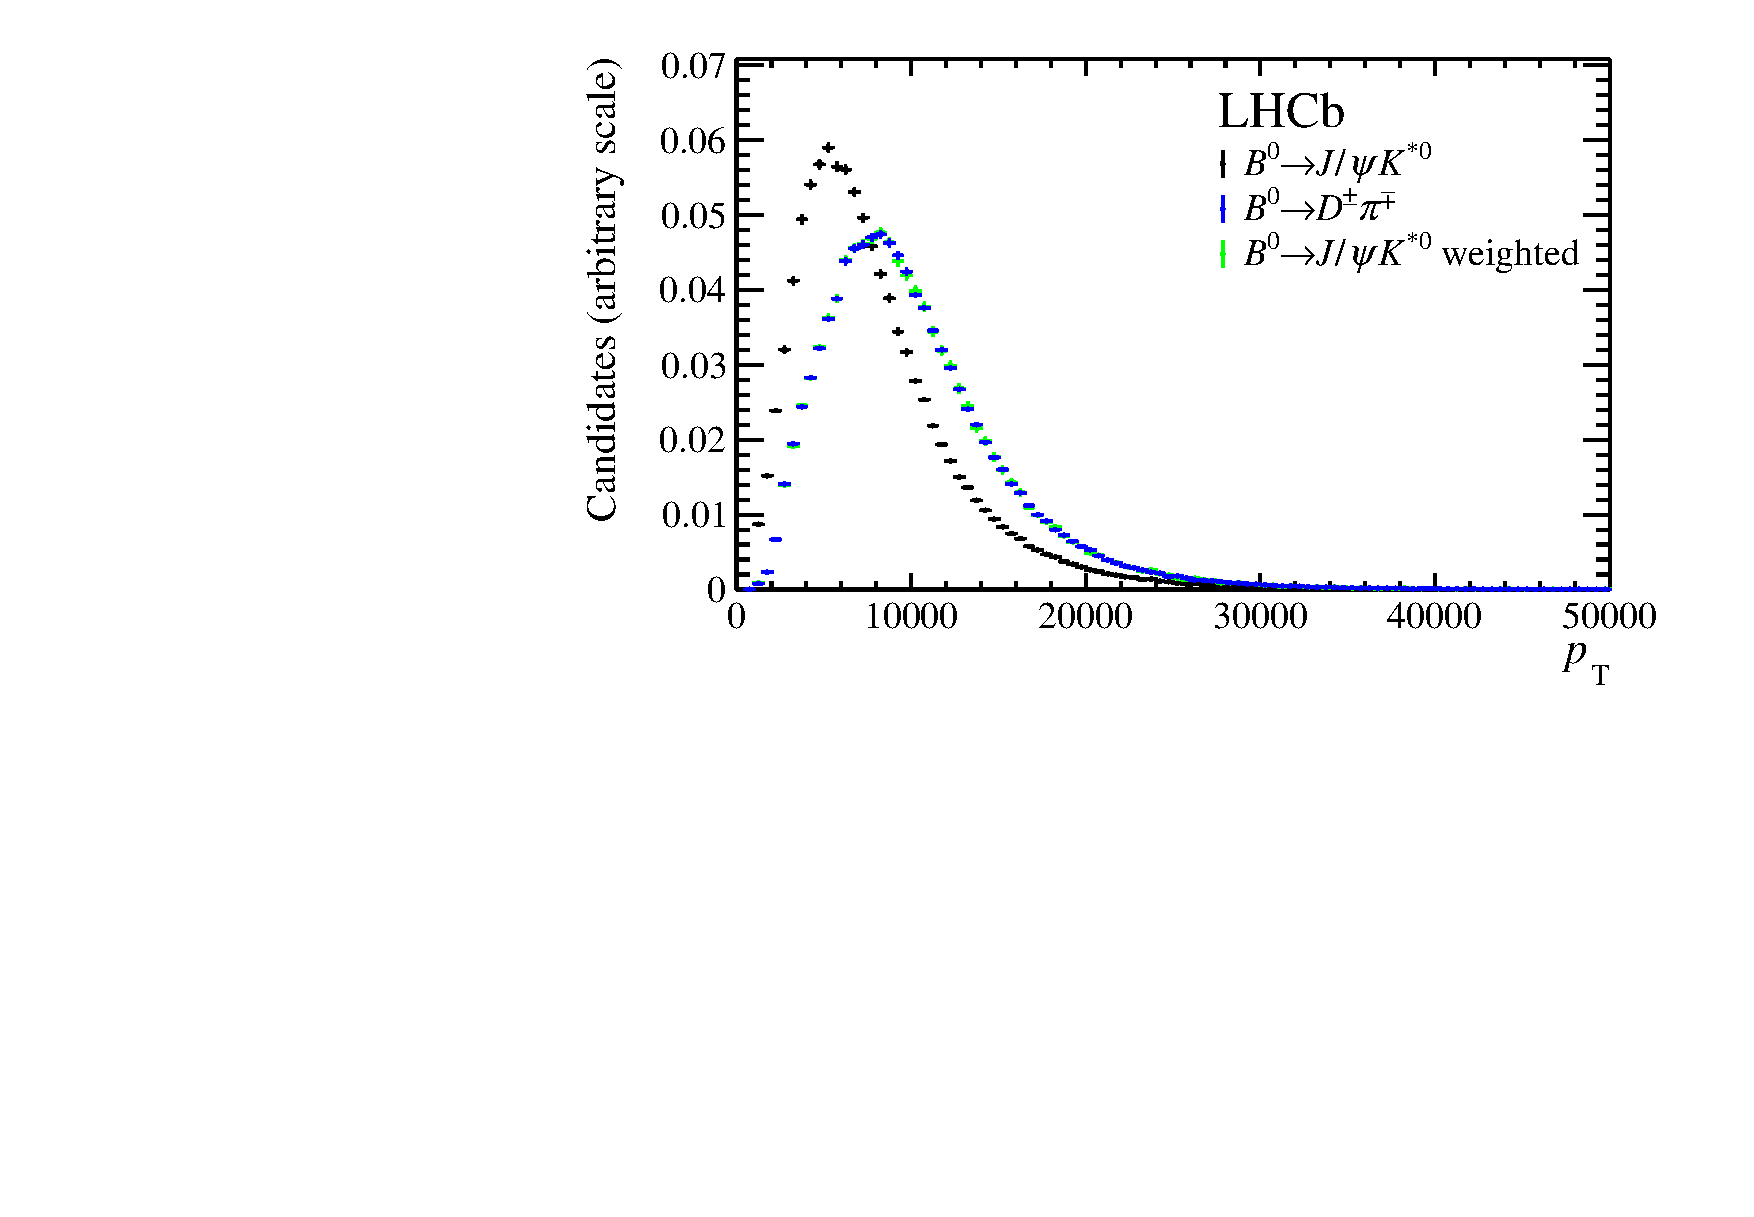
\includegraphics[width=0.48\textwidth]{08FlavourTagging/figs/pT_weighted.pdf}
    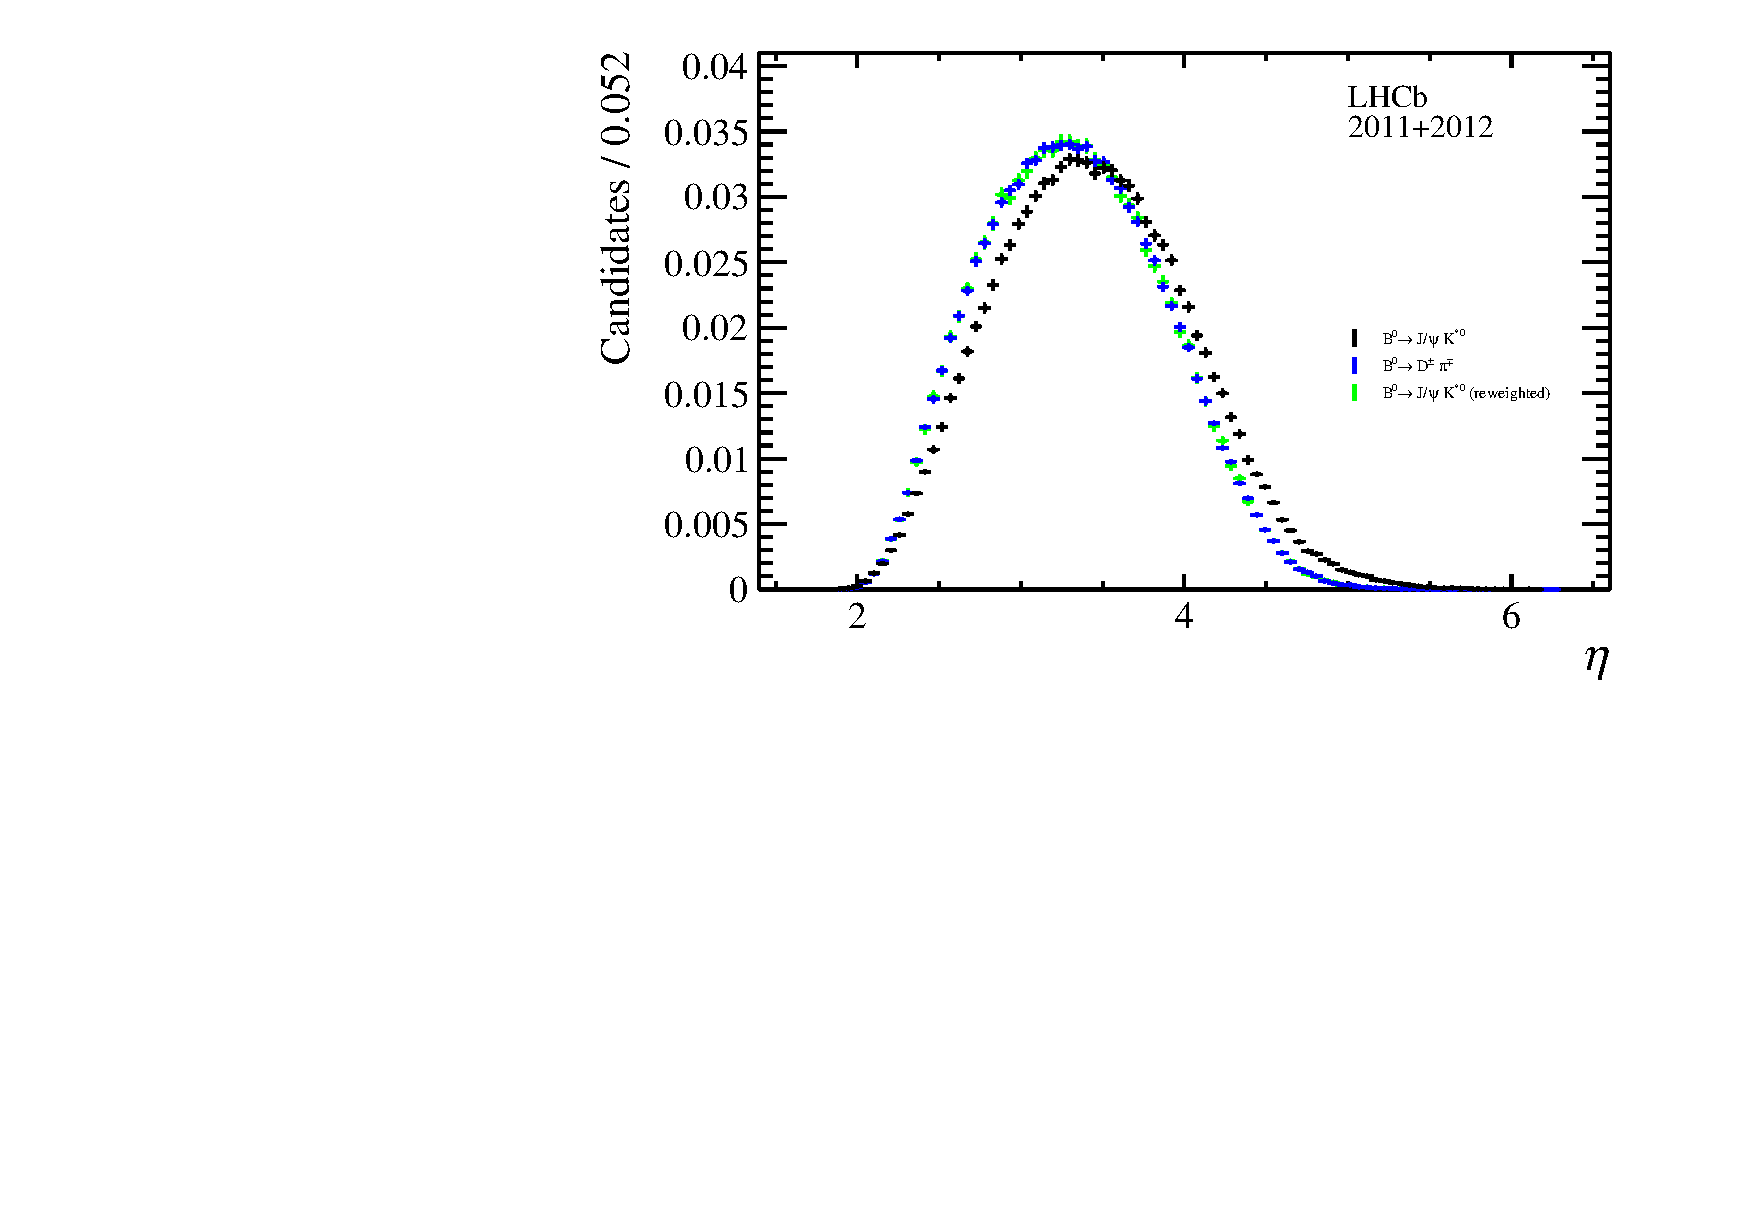
\includegraphics[width=0.48\textwidth]{08FlavourTagging/figs/eta_weighted.pdf}\\
    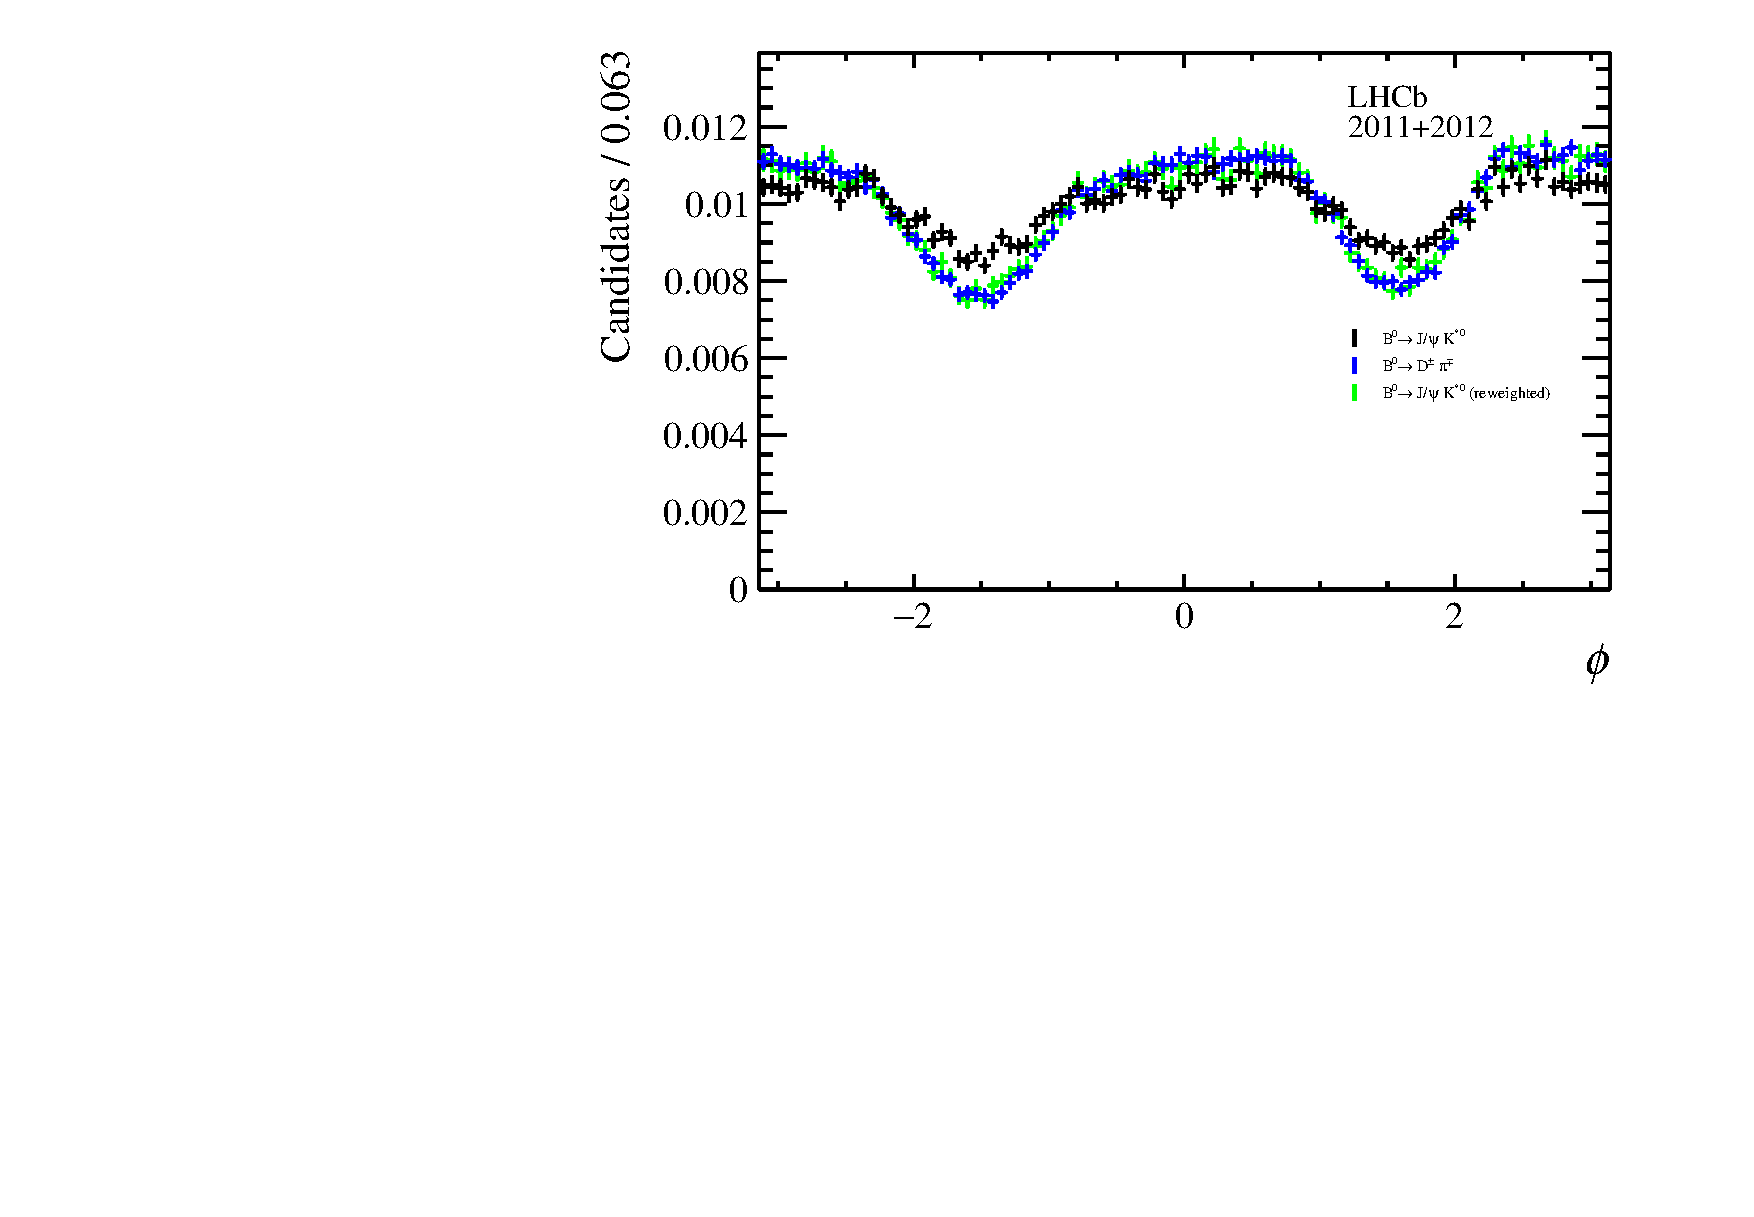
\includegraphics[width=0.48\textwidth]{08FlavourTagging/figs/phi_weighted.pdf}
    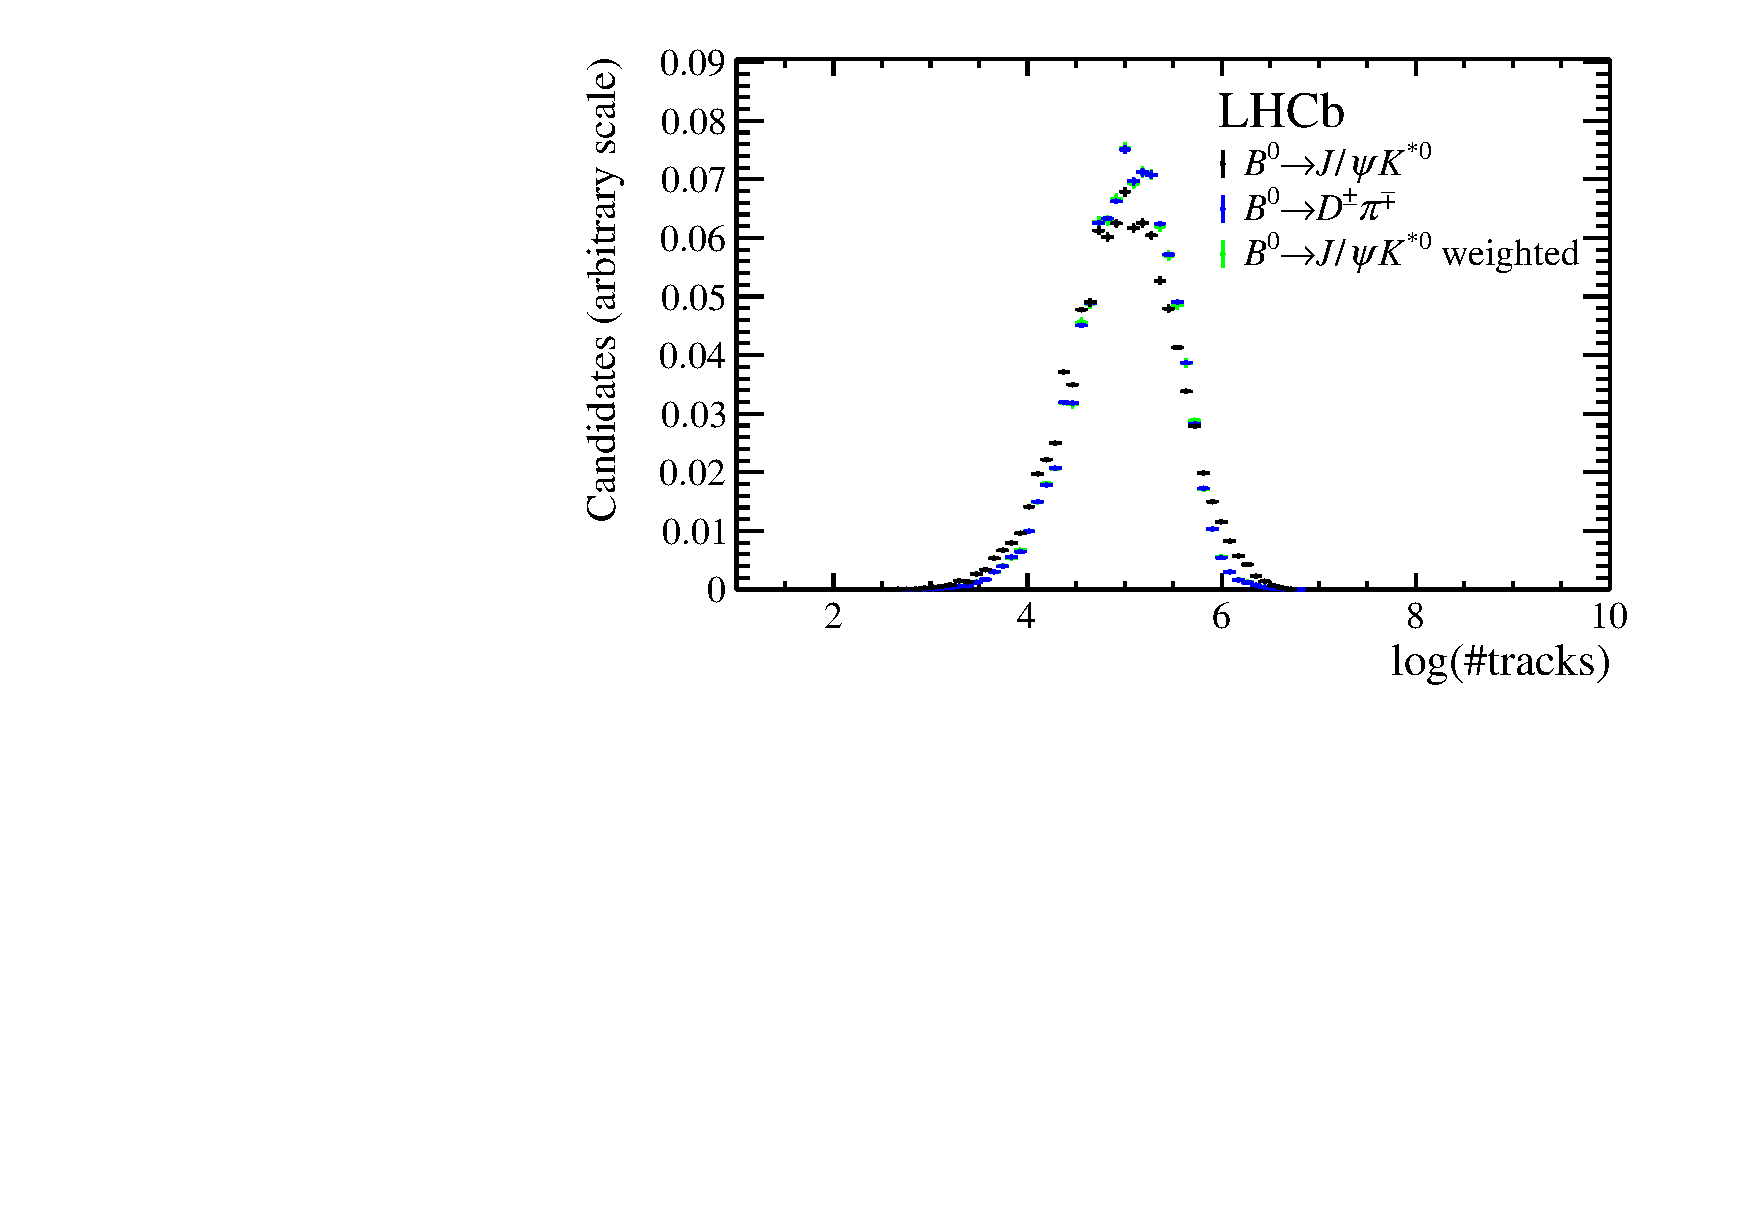
\includegraphics[width=0.48\textwidth]{08FlavourTagging/figs/nTracks_weighted.pdf}\\
    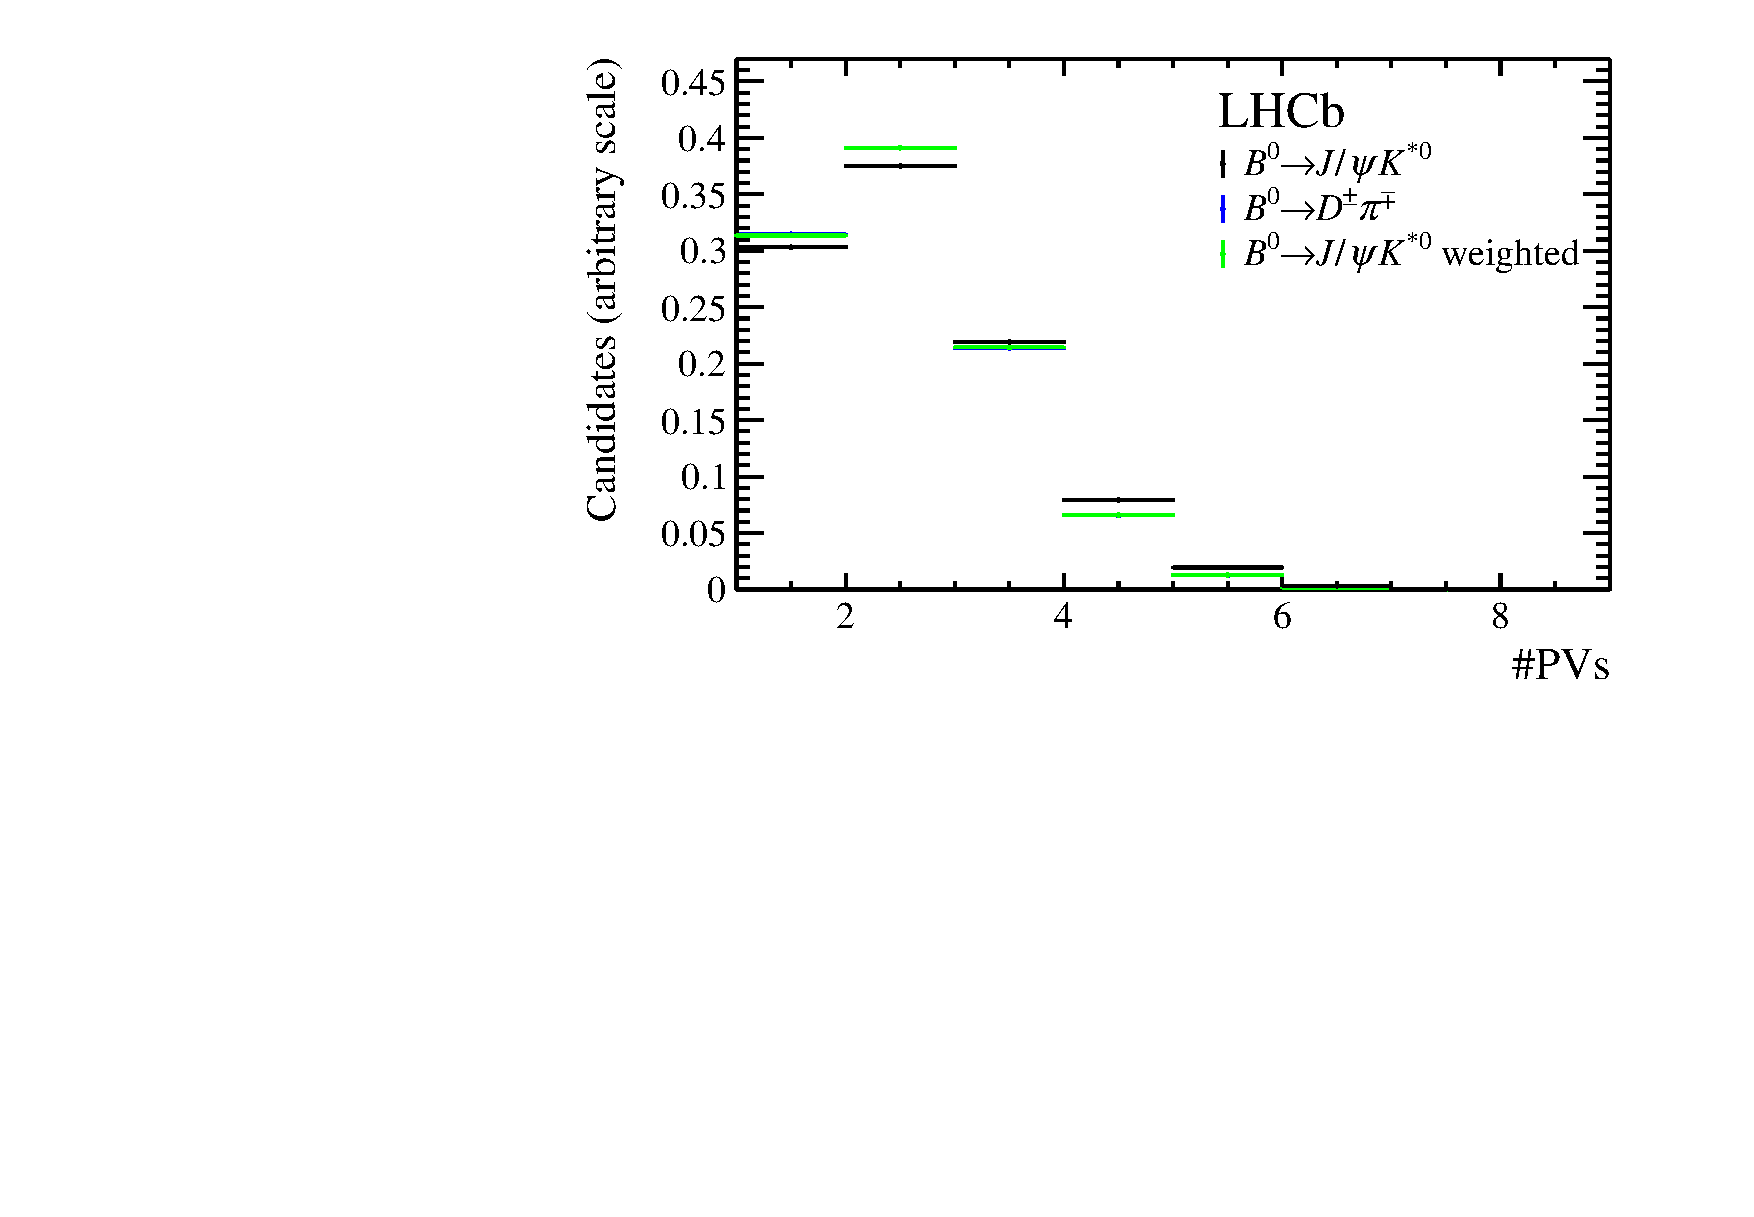
\includegraphics[width=0.48\textwidth]{08FlavourTagging/figs/nPV_weighted.pdf}
    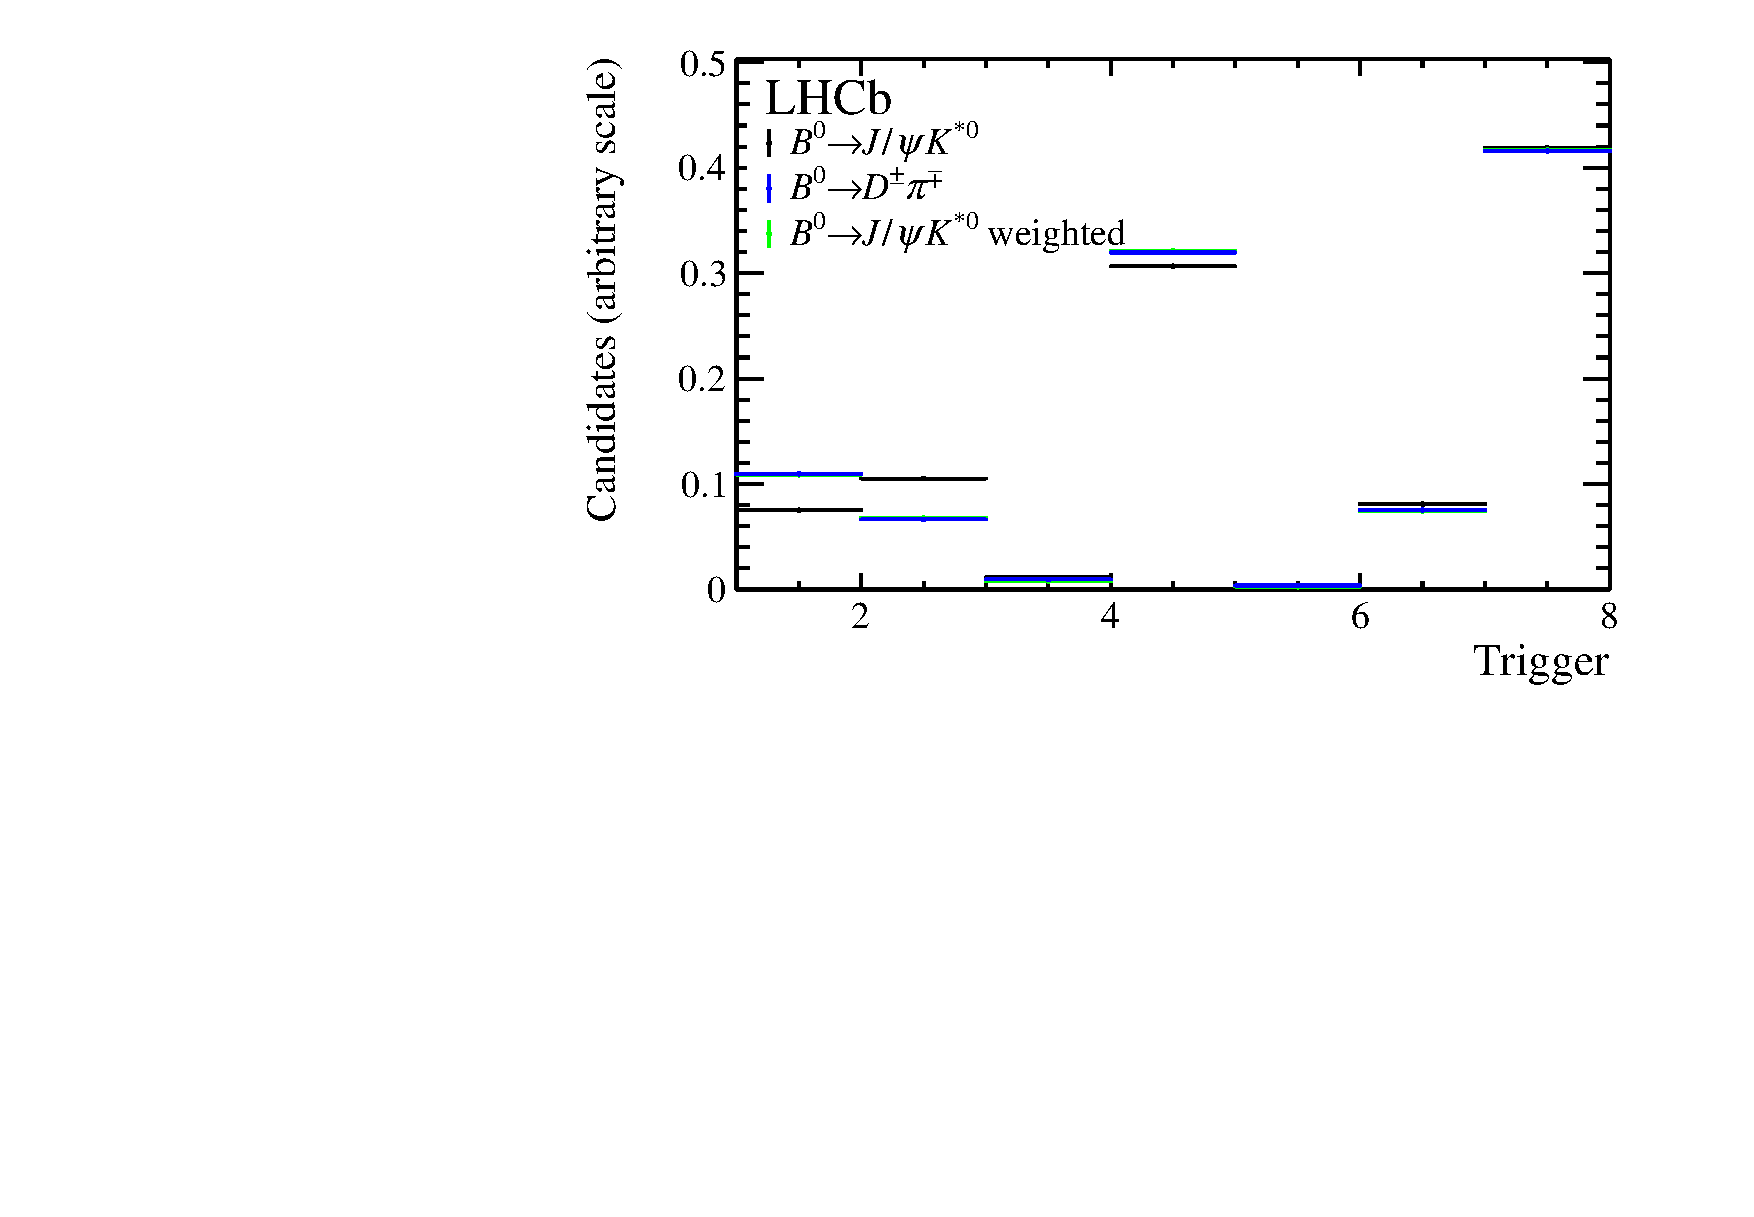
\includegraphics[width=0.48\textwidth]{08FlavourTagging/figs/Trigger_weighted.pdf}
    \caption{Left, top to bottom: Normalised \emph{sWeighted} distributions of the transverse momentum, azimuthal angle and number of tracks per event.
    Right, top to bottom: Normalised \emph{sWeighted} distributions of the pseudo-rapidity, logarithm of number of tracks per event and distribution of trigger decisions.}
    \label{fig:reweightingSS}
\end{figure}

\subsection{Retraining of the SS pion tagger}
\label{sec:retrainSSpion}

First the tagging particles have to fulfill a set of selection cuts, which are partly applied only to the tagging track and partly to the system of the tagging track and the \B candidate. These cuts have two aims:
First separating pions form other charged tracks in the event and second selecting particles which are in the same region of phase space as the \B candidate.
\begin{table}[tbp]
	\centering
	\caption{Selection cuts for the SS pion algorithm.
	The first set of cuts is applied only top the tagging-particle track, while the second set is applied to the \enquote{tagging-particle track+\B} system.}
	\begin{tabular}{cc}
		\toprule
		Variable & Cut \\
		\midrule
		transverse momentum \pt 											& $>\SI[per-mode=symbol]{0.4}{\GeVc}$ \\
		$\nicefrac{\text{IP}}{\sigma_{\text{IP}}}$							& $<4$ \\
		track ghost probability $g_{\text{prob}}$ 							& $<0.5$ \\
		\dllppi 															& $<5$ \\
		\dllkpi 															& $<5$ \\
		track $\nicefrac{\chi^2}{\text{ndof}}$ 								& $<5$ \\
		$\nicefrac{\text{IP}_{\text{PU}}}{\sigma_{\text{IP}_{\text{PU}}}}$ 	& $>3$ \\
		\midrule
		transverse momentum \pt 					& $>\SI{3}{\GeVc}$ \\
		$\Delta Q=m_{\B+\pion}-m_{\B}-m_{\pion}$ 	& $<\SI{1.2}{\GeVcc}$ \\
		$\Delta\eta'$								& $<1.2$ \\
		$\Delta\phi$								& $<1.1$ \\
		vertex $\chi^2$ 							& $<100$ \\
		\bottomrule
	\end{tabular}
	\label{tab:SSPionselectionCuts}
\end{table}
For each tagging-particle candidate passing the requirements shown in \cref{tab:SSPionselectionCuts}, the \B-meson gets a preliminary tag decision assigned, corresponding to the charge of the tagging particle (\mbox{$\pip\rightarrow d=+1$}, \mbox{$\pim\rightarrow d=-1$}).
The quantities $\Delta\eta'$ and $\Delta\phi$ describe the difference of pseudo-rapidity and azimuthal angle between the signal and tagging-particle track.
To further assure that the tagging-particle is also produced at the \ac{PV} with which the \B candidate has the smallest $\text{IP}\chi^2$, the impact parameter significance with the next \enquote{best} PV in the event (denoted as pile-up vertex) is used.
The corresponding quantities are $\nicefrac{\text{IP}}{\sigma_{\text{IP}}}$ and $\nicefrac{\text{IP}_{\text{PU}}}{\sigma_{\text{IP}_{\text{PU}}}}$, respectively.

Subsequent a BDT is trained to determine the mistag and to select the best tagging-particle candidate in events with more than one tagging-particle candidate passing  the selection in \cref{tab:SSPionselectionCuts}.
In the training, all candidates with the correct correlation between the preliminary tag and the \B-flavour are considered as signal, all with the wrong correlation are considered background.
A correct or wrong correlation for the SS pion algorithm means
\begin{align*}
	\text{Correct tag: }& \Bz\pip \text{ or } \Bzb\pim\,,\\
	\text{Wrong tag: }& \Bz\pim \text{ or } \Bzb\pip
\end{align*}
where only \B candidates with a decay time smaller than \SI{2.2}{\pico\second} are used in the BDT training to reduce the number of oscillated \B candidates.
The BDT further consists of \num{3000} trees with a maximum depth of two.
Each tree uses up to five of the input variables scanned at 30 points to find the optimal cut point.
As boost algorithm AdaBoost~\cite{AdaBoost} is chosen with a boost factor of $\beta=0.005$.
A list of the input variables is given in \cref{tab:BDTInputSSPion}.
\begin{table}[tbp]
	\centering
	\caption{List of input variables used in the training of the BDT for the SS pion tagger.
	The quantity $\mathrm{ProbNNK}$ is the probability for a particle to be a kaon, calculated by an artificial neural network using information from the \lhcb PID system.
	The momentum of a particle is denoted as $p$.}
	\begin{tabular}{cc}
		\toprule
		\multirow{6}{*}{tagging-particle inputs} 	& $\log\left(\pt\right)$ \\
													& $\log\left(p\right)$ \\
													& $\log\left(\text{IP}/\sigma_\text{IP}\right)$\\
													& $\log\left(g_\text{prob}\right)$\\
													& $\log\left(\text{track} \nicefrac{\chi^2}{\text{ndof}}\right)$ \\
													& $\log\left(\text{ProbNNK}\right)$\\
		\midrule
		\multirow{5}{*}{tagging-particle + $\Bz$ inputs}	& $\Delta Q$\\
															& $\Delta R$\\
															& $\log\left(\Delta\eta'\right)$\\
															& $\log\left(\Delta\phi\right)$\\
															& $\log\left(\pt\right)$\\
		\midrule
		\multirow{1}{*}{event properties}	& PVndof\\
		\bottomrule
	\end{tabular}
	\label{tab:BDTInputSSPion}
\end{table}
\begin{figure}[tbp]
	\begin{center}
		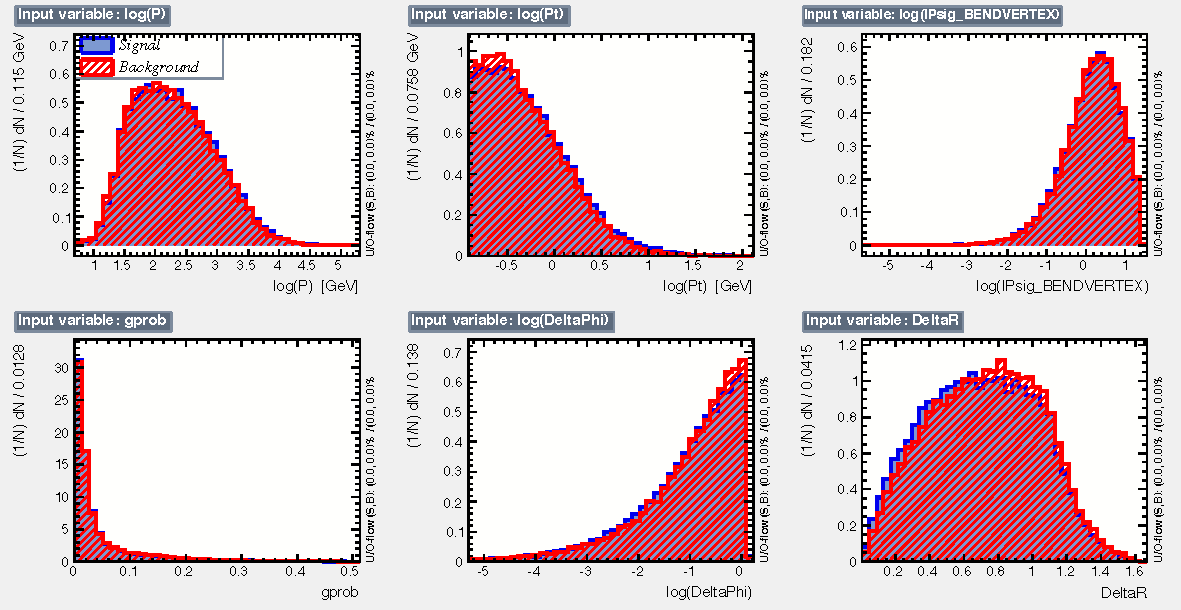
\includegraphics[width=0.8\textwidth]{08FlavourTagging/figs/SSpionBDT_input1.pdf}\\
		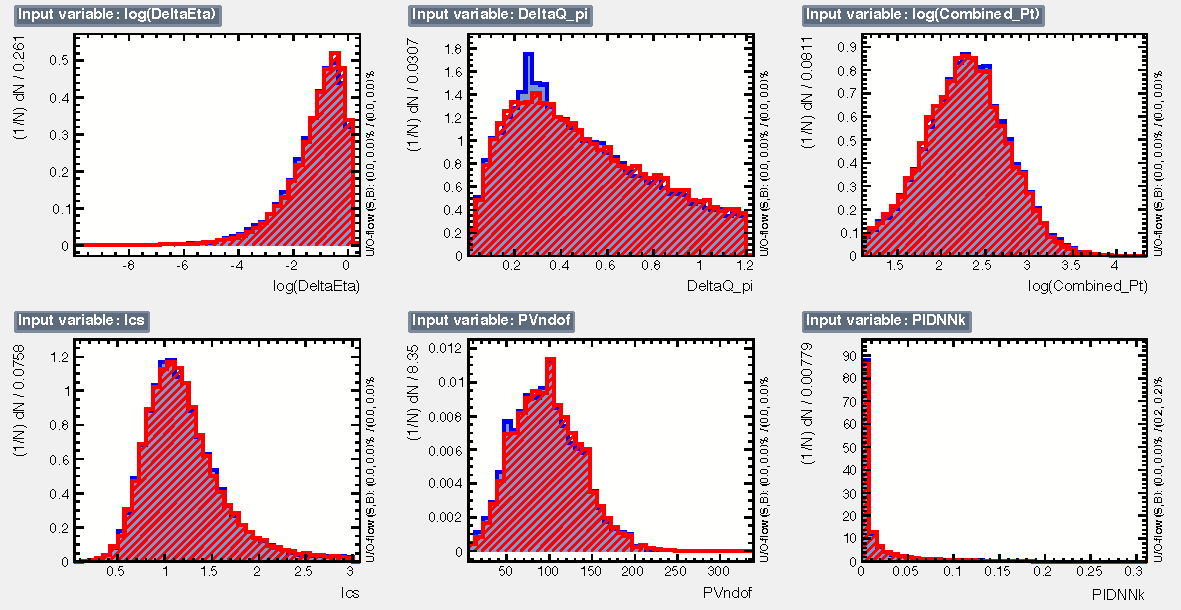
\includegraphics[width=0.8\textwidth]{08FlavourTagging/figs/SSpionBDT_input2.pdf}
	\end{center}
	\caption{Distributions of the input variables used in the BDT training.
	The blue curve represents the right charge correlation while the red curve corresponds to the wrong ones.}
	\label{fig:BDTInputSSPion}
\end{figure}
Most of these variables were already used in the selection, PVndof is the number of degrees of freedom in the fit to determine the position of the \ac{PV} and $\Delta R=\sqrt{\Delta\phi^2+\Delta\eta'^2}$.
Moreover a logarithmic transformation is applied to some of the input variables to improve the performance of the BDT.
As one can see in \cref{fig:BDTInputSSPion} the distributions of the signal and background samples are quite similar.
This small, but significant difference is propagated to the distribution of the BDT response as shown in \cref{fig:BDTovertrainSSPion}.
\begin{figure}[tbp]
	\begin{center}
		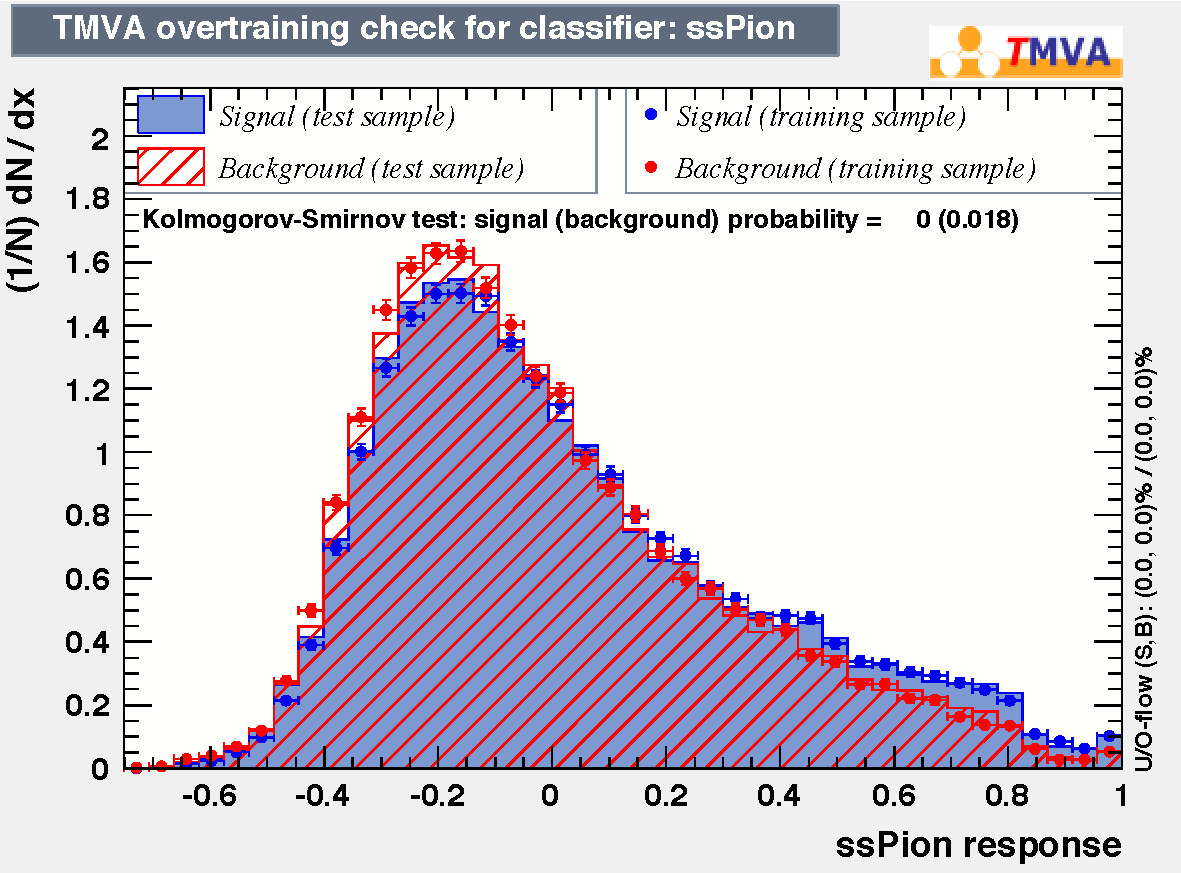
\includegraphics[width=0.6\textwidth]{08FlavourTagging/figs/SSPionBDT_overtrain.pdf}
	\end{center}
	\caption{Output of the SS pion BDT ($\alpha^{\text{SS}\pion}_\text{BDT}$).
	The blue distribution represents the right charge correlated tracks while the red distribution corresponds to the wrong charge correlated tracks.}
	\label{fig:BDTovertrainSSPion}
\end{figure}
For events with more than one tagging particle, the best one is identified as the particle with the largest BDT output.

Subsequently, due to the flavour oscillations, a time-dependent analysis is necessary to transform the BDT response into a mistag.
For this, an unbinded maximum-likelhihood fit to the decay-time $t$, the tag decisions $d$ and the mixing state $\xi$ is performed.
The mixing state takes values of $+1$ when the \B-meson flavour at decay is the same as the tag decision and $-1$ otherwise.
As the fit is performed to the \emph{sWeighted} decay-time distribution the describing PDF consists only of a signal-component
\begin{equation}
\mathcal{M}(t;d,\xi)=\mathcal{N}a(t)e^{-t'/\tau}\left(\left(1-d\Delta\omega\right)+\xi\left(1-2\omega\right)\cos\!\left(\dm t'\right)\right)\otimes\mathcal{R}(t-t')\label{eq:mixPDF}
\end{equation}
where $\mathcal{N}$ is a normalisation factor and $\omega$ and $\Delta\omega$ are the mistag and mistag difference for initial \Bz- and \Bzb-mesons, respectively.
$\mathcal{R}(t-t')$ describes an average decay time resolution of \SI{50}{\femto\second}.
The lifetime is constrained by means of a Gaussian function to be $\tau=\num{1.518\pm0.004}$ what allows to float the parameters of the cubic-splines describing the decay-time acceptance $a(t)$.
These cubic-splines have five knots placed at $[0.2, 0.25, 2.0, 13.8, 14.5]\,$\si{\pico\second} (more details in \cref{sec:acceptance}).
At first the fit is performed in bins of the BDT response to determine pairs of the average BDT response and mistag.
These pairs are then used to determine the functional form of the transformation and a $3^{\text{rd}}$ order polynomial of the form
\begin{equation}
\omega\left(\alpha^{\text{SS}\pion}_\text{BDT}\right)=b_0+b_1\times\alpha^{\text{SS}\pion}_\text{BDT}+b_2\times{\alpha^{\text{SS}\pion}_\text{BDT}}^2+b_3\times{\alpha^{\text{SS}\pion}_\text{BDT}}^3\label{eq:tranformfunc}
\end{equation}
is found to describe the relation well.
However, to determine the final transformation parameters, an unbinned fit, where the mistag is parametrised directly in the PDF, is performed.
Figure \eqref{fig:MixingSSPion} shows the projected mixing asymmetry from the decay-time fit, defined as
\begin{equation}
A(t)=\frac{N_{\text{unmix}}(t)-N_{\text{mix}}(t)}{N_{\text{unmix}}(t)+N_{\text{mix}}(t)}\propto\left(1-2\omega\right)\cos\!\left(\dm t\right)
\end{equation}
where $N_{\text{unmix}}(t)$ and $N_{\text{mix}}(t)$ are the number of unmixed  and mixed \Bz candidates for a decay time $t$, respectively.
\begin{figure}[tbp]
	\begin{center}
		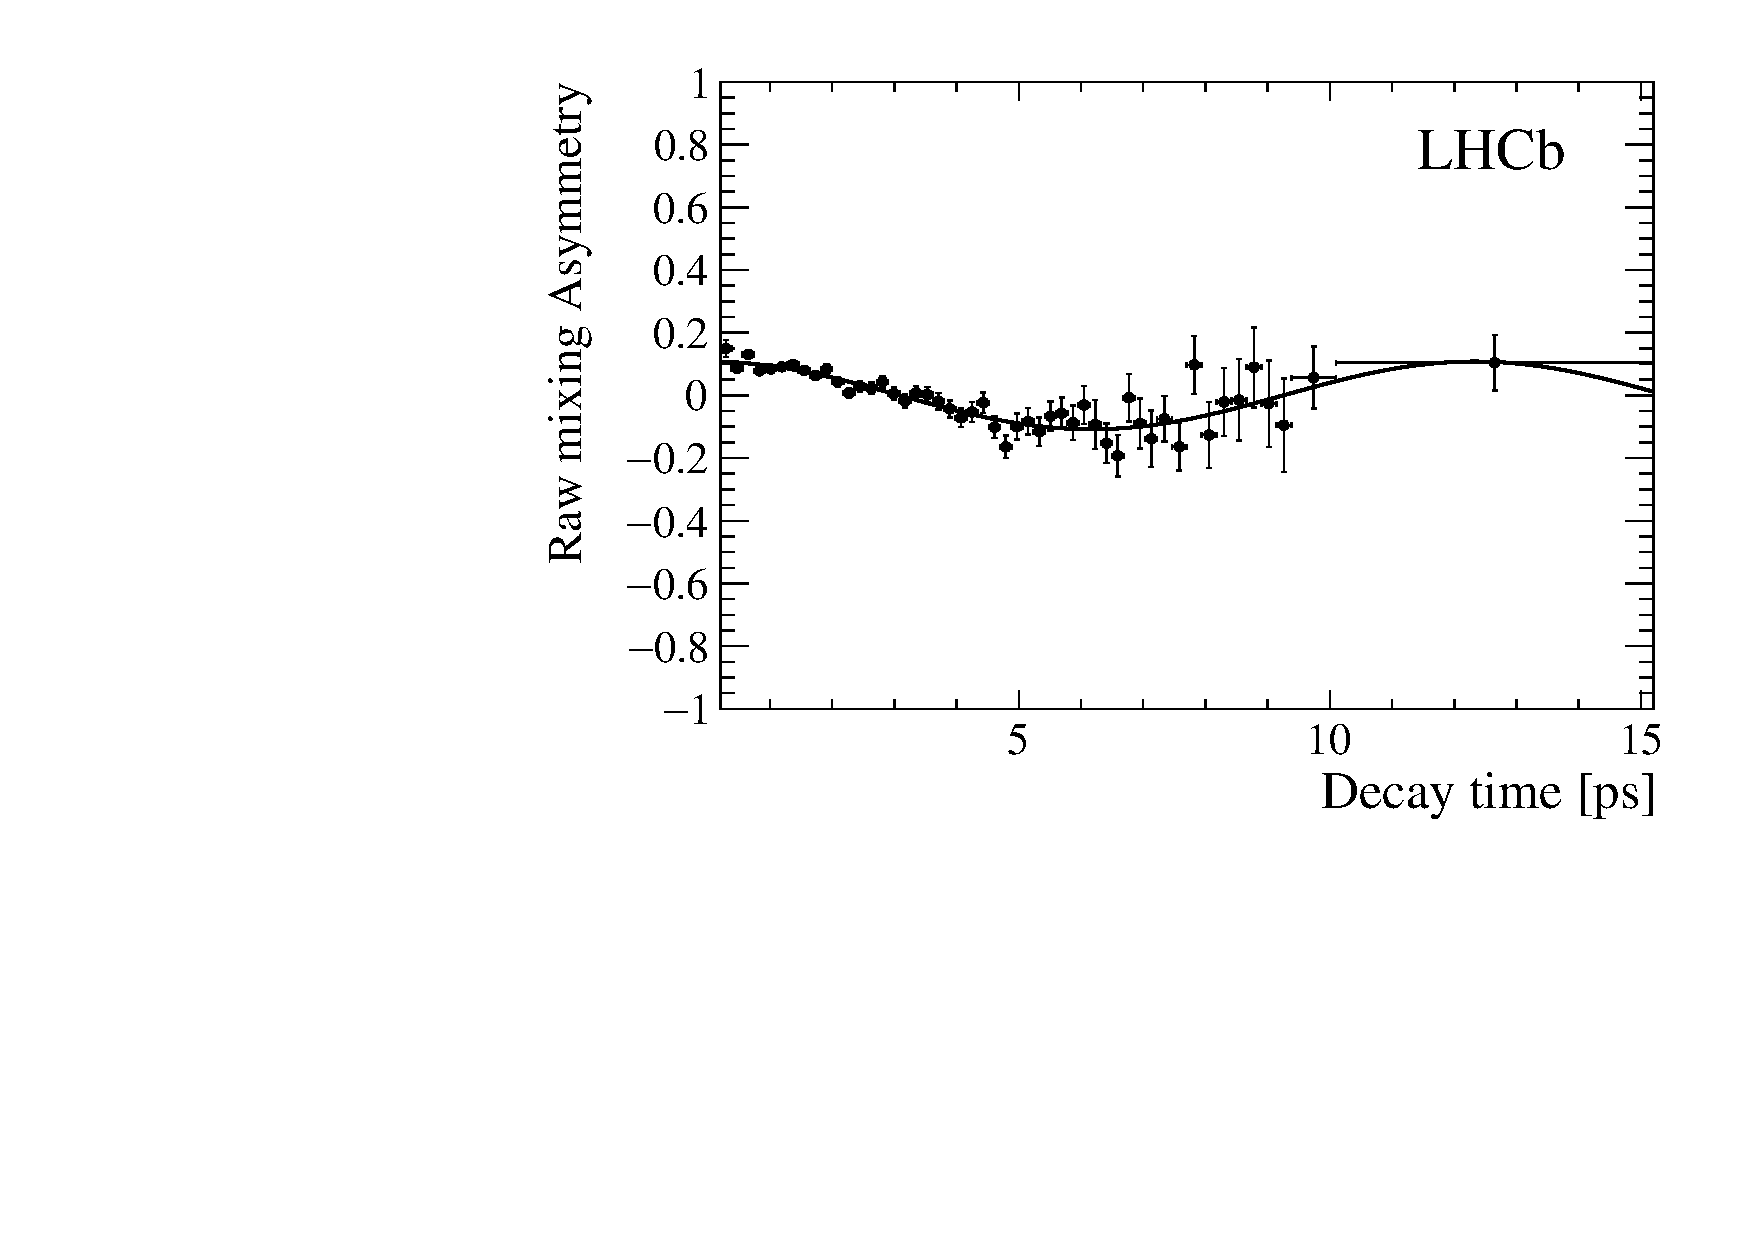
\includegraphics[width=0.6\textwidth]{08FlavourTagging/figs/Asymmetry_SSPion.pdf}
	\end{center}
	\caption{Mixing asymmetry for $\Bz\!\to\jpsi\Kstarz$ candidates tagged by the SS pion tagger.
	The curve overlaid is the fit projection of the decay-time fit.}
	\label{fig:MixingSSPion}
\end{figure}
The resulting transformation parameters are given in \cref{tab:transformationSSPion}, while \cref{fig:transformationSSPion} shows the corresponding $3^{\text{rd}}$ order polynomial.
\begin{table}[tbp]
	\centering
	\caption{Final transformation parameters for the BDT responst of the SS pion tagger.}
	\begin{tabular}{cccc}
		\toprule
		$b_0$ & $b_1$ & $b_2$ & $b_3$ \\
		\midrule
		\num{0.469\pm0.003} & \num{-0.066\pm0.012} & \num{-0.022\pm0.048} & \num{-0.026\pm0.056} \\
		\bottomrule
	\end{tabular}
	\label{tab:transformationSSPion}
\end{table}
\begin{figure}[tbp]
	\begin{center}
		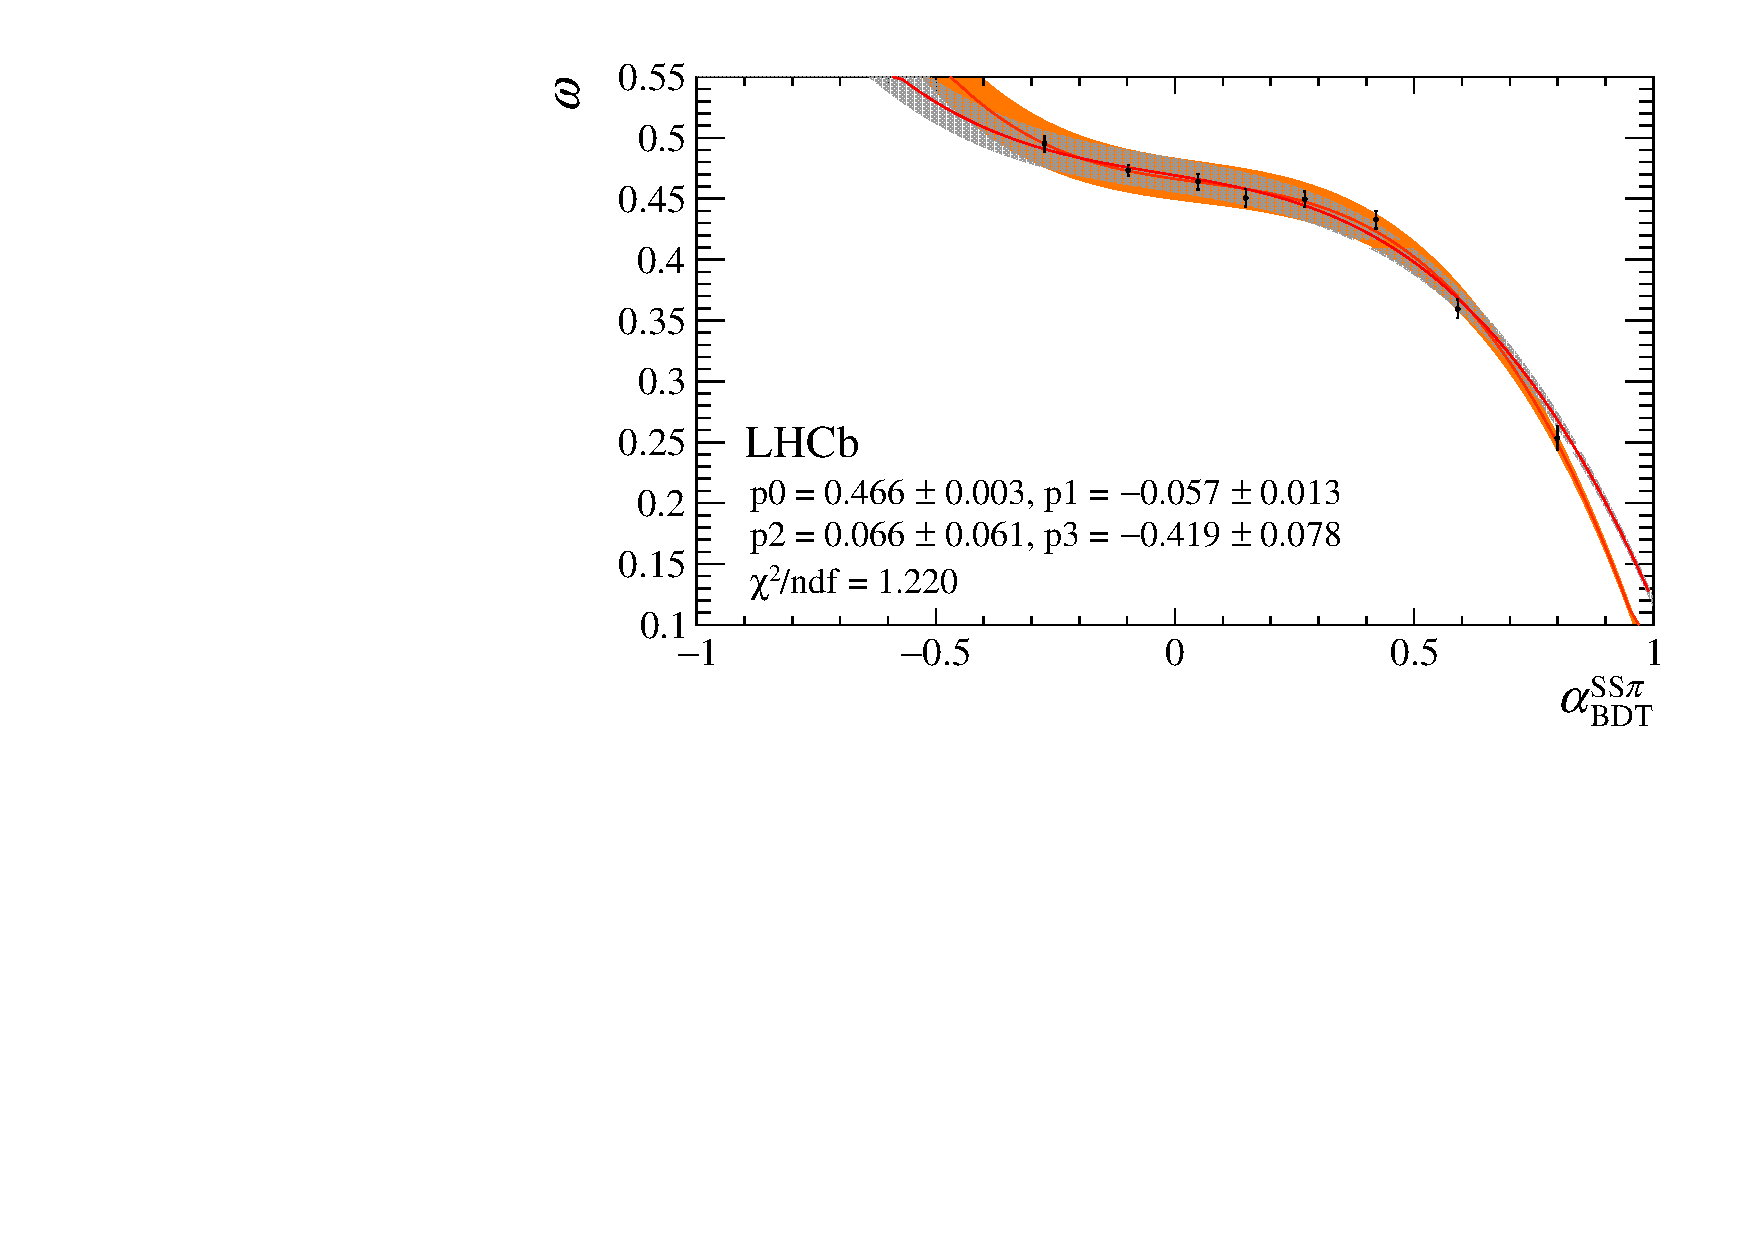
\includegraphics[width=0.6\textwidth]{08FlavourTagging/figs/SSPionBDTTrafo.pdf}
	\end{center}
	\caption{Polynomial curve of $\omega$ versus $\alpha^{\text{SS}\pion}_\text{BDT}$ on the first two thirds of the $\Bz\!\to\jpsi\Kstarz$ data sample.
	The fit from the binned approach is shown in orange, the curved of the nominal unbinned method is shown in grey .
	The parameter values in the plot correspond to the orange curve/binned approach.}
	\label{fig:transformationSSPion}
\end{figure}
Using this transformation for each \Bz candidate the mistag final mistag $\eta$ is calculated.
In case the computed mistag $\eta'$ is larger than \num{0.5}, the tag decision is inverted and the final mistag is calculated as $\eta=1-\eta'$.

\subsection{Retraining of the SS proton tagger}
\label{sec:retrainSSproton}

The procedure for tuning the SS proton tagger BDT and transforming the BDT response is very similar to the one described in \cref{sec:retrainSSpion} for the SS pion tagger.

Besides pions, protons, which have a correlation with the initial flavour of the \B-meson, may also be formed in the hadronisation process.
These tagging-proton candidates must first meet a set of requirements for the proton track itself and the system of the tagging-proton candidate and the \B-meson.
These cuts are listed in \cref{tab:selectionSSProton}.
The correlation between charge of the proton and the \B-meson flavour for the SS proton tagger is as follows:
\begin{align*}
	\text{Correct tag: }& \Bz\antiproton \text{ or } \Bzb\proton\,,\\
	\text{Wrong tag: }& \Bz\proton \text{ or } \Bzb\antiproton\,.
\end{align*}
Based on the charge of the selected particles, consequently a preliminary tag is assigned to the \B candidates ($\proton\rightarrow  d=-1$, $\antiproton\rightarrow d=+1$).
\begin{table}[bp]
	\centering
	\caption{Selection cuts for the SS proton algorithm.
	The first set of cuts is applied only on the tagging-particle track, while the second set is applied to the \enquote{tagging-particle track+\B} system.
	The quantity $\Delta Q$ is defined as $\Delta Q=m_{\B+\proton}-m_{\B}-m_{\proton}$.}
	\begin{tabular}{cccccc}
		\toprule
		Variable & \pt & $\text{IP}/\sigma_\text{IP}$ & $g_\text{prob}$ & $\dllppi$ & $\text{IP}_\text{PU}/\sigma_{\text{IP}_\text{PU}}$ \\
		Cut & $>\SI{0.4}{\GeVc}$ & $<4$ & $<0.5$ & $>5$ & $>3$ \\
		\midrule
		Variable & \pt & $\Delta Q$ & $\Delta\eta'$ & $\Delta\phi$  & vertex $\chi^2$ \\
		Cut & $>\SI{3}{\GeVc}$ & $<\SI{1.2}{\GeVcc}$ & $<1.2$ & $<1.1$ & $<100$ \\
		\bottomrule
	\end{tabular}
	\label{tab:selectionSSProton}
\end{table}

Here it is important to note that the correlation is the exact opposite to the one of the SS pion tagger.
As a consequence, a misidentification of pions and protons would lead to a degraded performance of both taggers and the requirement on \dllppi is chosen exactly the opposite for both algorithms.
Furthermore, this requirement reduces the correlation between both taggers as the set of selected tagging particles are completely disjoint.

In the same way as for the SS pion tagger, proton candidates with the correct charge correlation with the flavor of the initial \B-meson are assumed to be signal while proton candidates with the incorrect charge correlation are considered as background for the BDT training.
The input variables for the BDT are listed in \cref{tab:BDTInputSSProton}, most of them again already used for the selection.
\begin{table}[tbp]
	\centering
	\caption{List of input variables used in the training of the BDT for the SS proton tagger.
	The momentum of a particle is denoted as $p$.}
	\begin{tabular}{cc}
		\toprule
		\multirow{4}{*}{tagging particle inputs} 	&	$\log\left(\pt\right)$ \\
													&	$\log\left(p\right)$\\
													&	$\log\left(\text{IP}/\sigma_\text{IP}\right)$\\
													&	$\log\left(\dllppi\right)$\\
		\midrule
		\multirow{3}{*}{tagging particle + $\Bz$ inputs} 	& $\Delta Q$\\
															& $\Delta R$\\
															& $\log\left(\Delta\eta'\right)$\\
		\midrule
		\multirow{1}{*}{event properties} 	& PVndof\\
		\bottomrule
	\end{tabular}
	\label{tab:BDTInputSSProton}
\end{table}
As in \cref{sec:retrainSSpion}, the distributions of the input variables are very similar for the datasets considered as signal and background.
Again, only \B candidates with a decay time below \SI{2.2}{\pico\second} are used for the BDT training and some of the input variables are logarithmically transformed to improve the performance.
All further configurations of the BDT are same as described in \cref{sec:retrainSSpion}, in \cref{fig:SSProtonBDTOutput} the BDT response is shown.
\begin{figure}[htbp]
	\begin{center}
		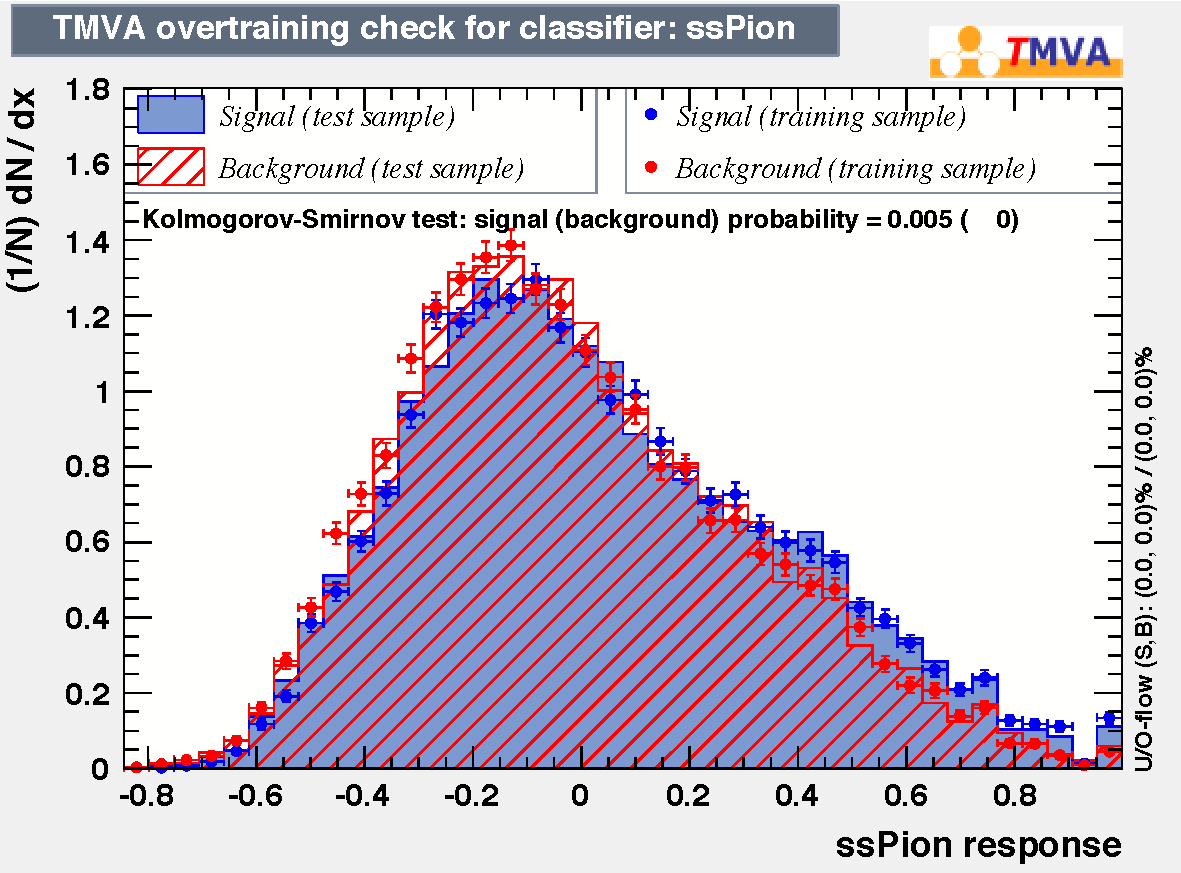
\includegraphics[width=0.6\textwidth]{08FlavourTagging/figs/SSProton_overtrain.pdf}
	\end{center}
	\caption{Output of the SS proton BDT ($\alpha^{\text{SS}\proton}_\text{BDT}$).
	The blue distribution represents the right charge correlated tracks while the red distribution corresponds to the wrong charge correlated tracks.}
	\label{fig:SSProtonBDTOutput}
\end{figure}
Again, a small but significant separation power of the BDT can be seen.
In addition, the test and training samples show some small differences, which probably are a result of a slight overtraining.
However, possible effects arrising due to this are corrected when transforming and calibrating the BDT response.
As for the SS pion algorithm, in case of multiple tagging-proton candidates per event the tag decision and the mistag are defined by the candidate with the largest BDT output.

To determine the relation between the mistag and the BDT output, a time-dependent mixing analysis is performed.
This means, an unbinned maximum-likelihood fit to the distribution of the decay-time $t$, the tag decision $d$ and the mixing state $\xi$ is done.
Since the \emph{sWeigthed} distributions are used for the fit again, only the signal component must be described with the PDF from \cref{eq:mixPDF}.
Firstly the functional relation between the mistag and $\alpha^{\text{SS}\proton}_\text{BDT}$ is determined with a binned fit in the BDT output $\alpha^{\text{SS}\proton}_\text{BDT}$.
Again a $3^{\text{rd}}$ order polynomial as described in \cref{eq:tranformfunc} describes the data well.
An unbinned fit, in which the mistag is parametrised directly in the PDF, finally provides the final transformation parameters, which can be found in \cref{tab:transformSSProton}.
\begin{table}[tbp]
	\centering
	\caption{Final transformation parameters for the BDT response of the SS proton tagger.}
	\begin{tabular}{cccc}
		\toprule
		$b_0$ & $b_1$ & $b_2$ & $b_3$ \\
		\midrule
		\num{0.479\pm0.004} & \num{-0.097\pm0.016} & \num{0.009\pm0.043} & \num{-0.215\pm0.064} \\
		\bottomrule
	\end{tabular}
	\label{tab:transformSSProton}
\end{table}
Figure \ref{fig:MixasymmetrieSSProton} shows the time-dependent mixing asymmetry for the SS proton tagger, the transformation functions of the binned and unbinned approach are presented in \cref{fig:transformationSSProton}.
\begin{figure}[tbp]
	\begin{center}
		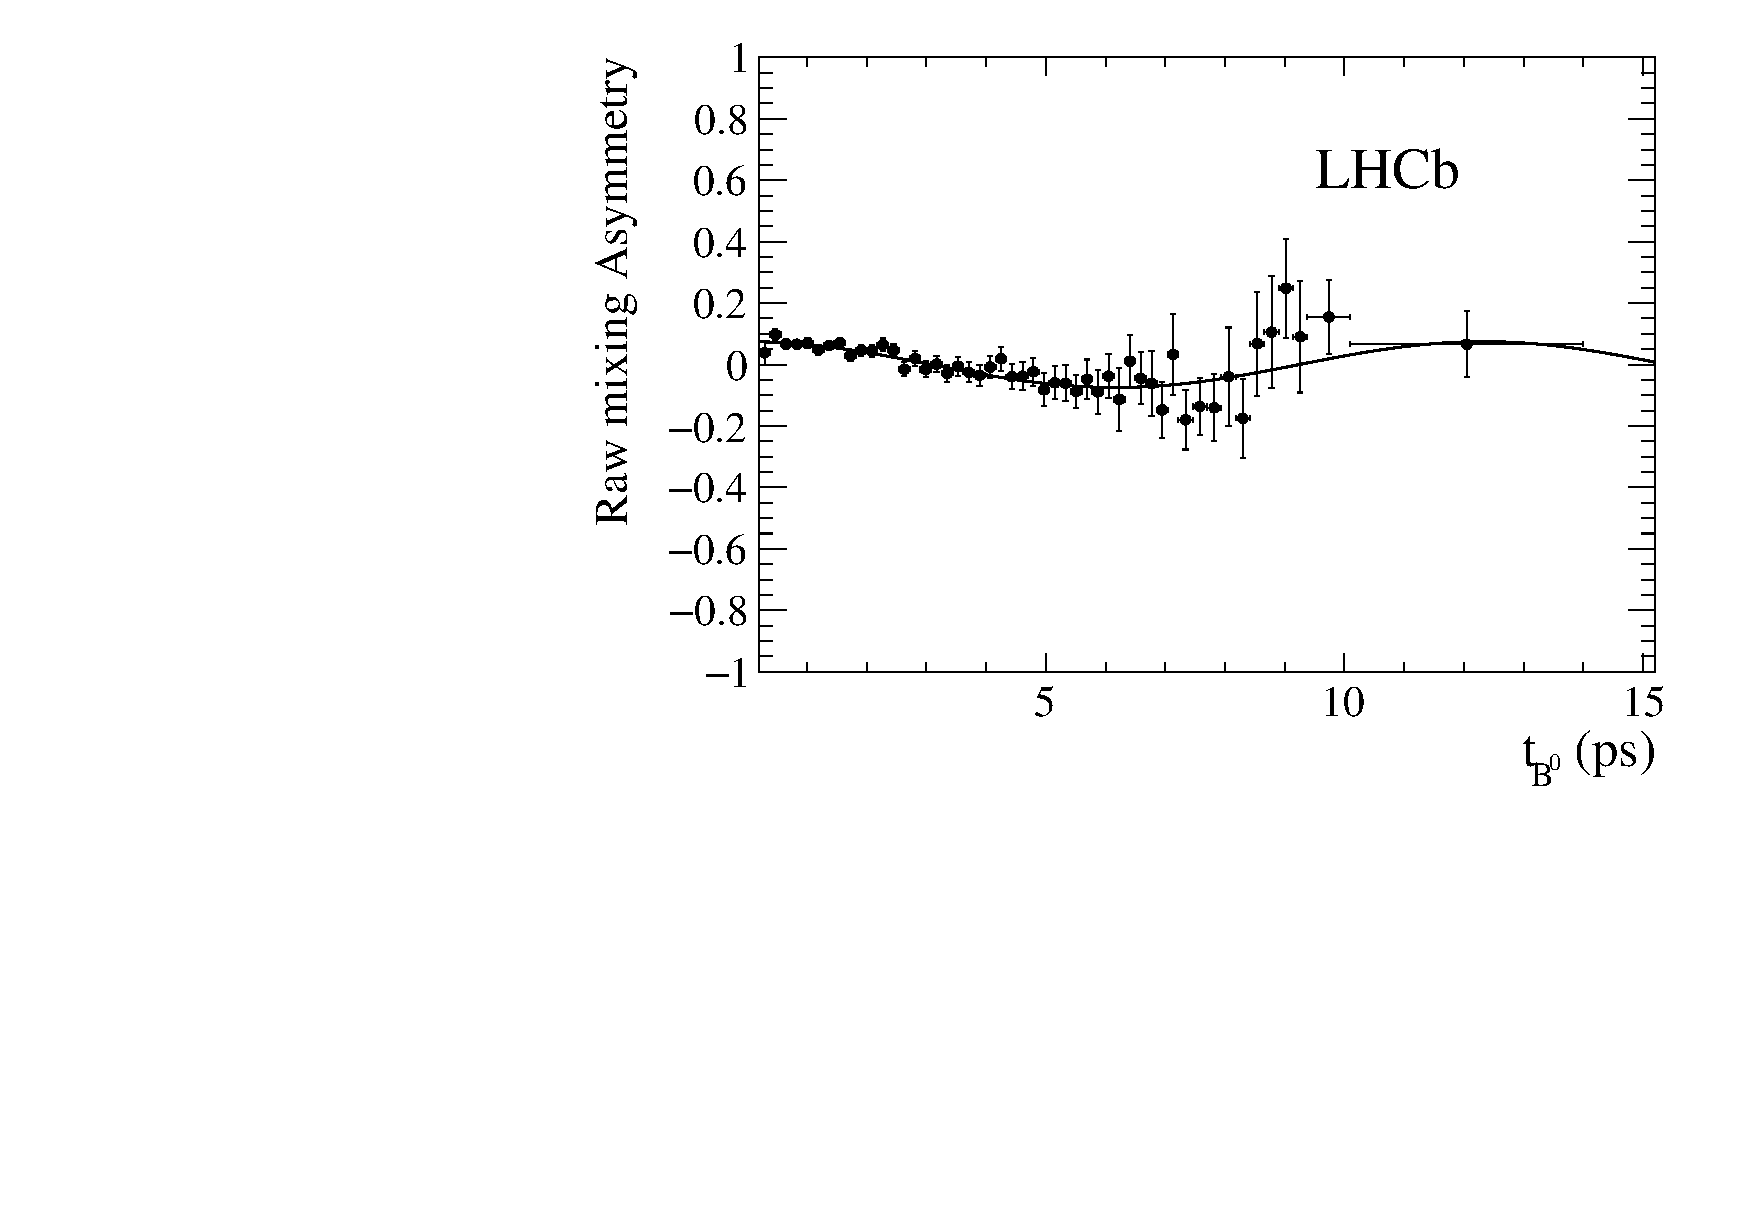
\includegraphics[width=0.6\textwidth]{08FlavourTagging/figs/Asymmetry_SSProton.pdf}
	\end{center}
	\caption{Mixing asymmetry for $\Bz\!\to\jpsi\Kstarz$ candidates tagged by the SS proton tagger.
	The curve overlaid is the fit projection of the decay-time fit.}
	\label{fig:MixasymmetrieSSProton}
\end{figure}
\begin{figure}[tbp]
	\begin{center}
		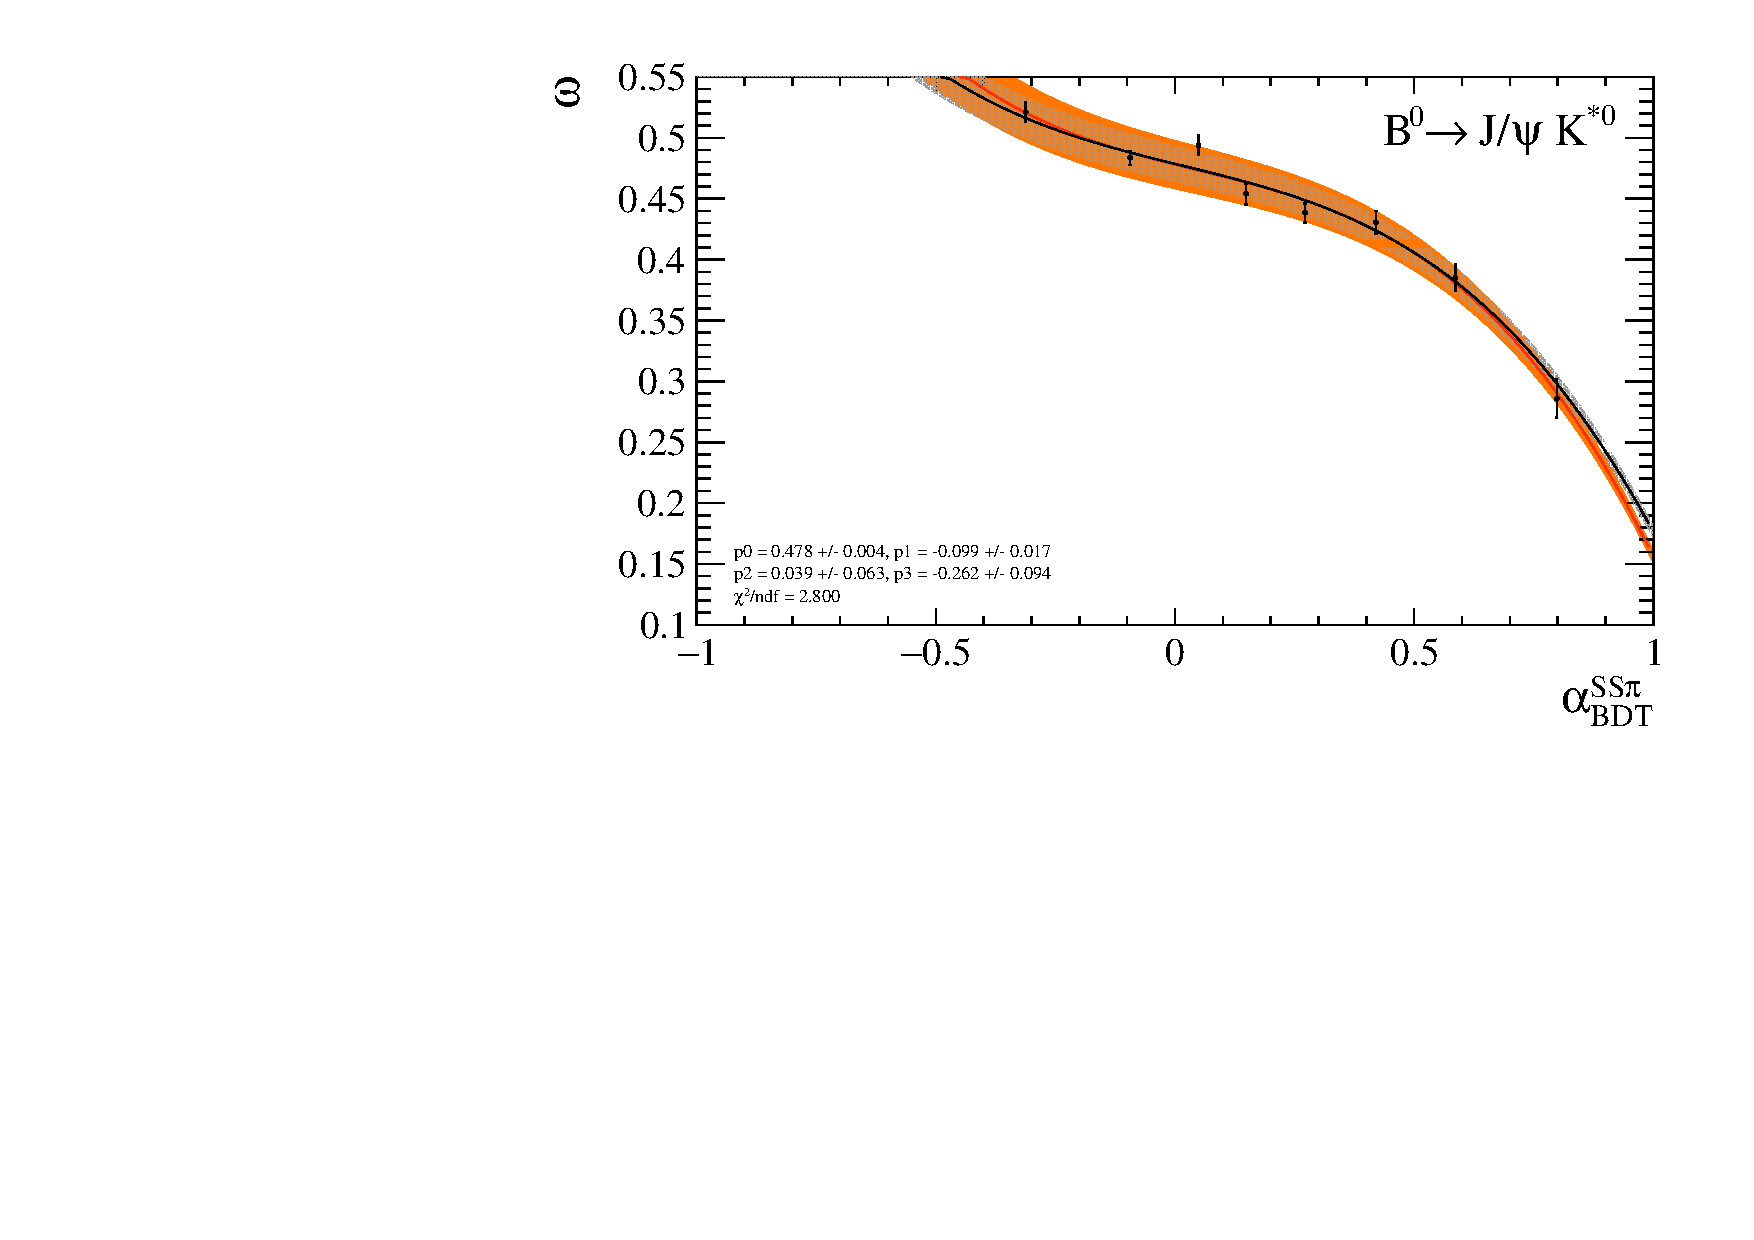
\includegraphics[width=0.6\textwidth]{08FlavourTagging/figs/SSProtonBDTTrafo.pdf}
	\end{center}
	\caption{Polynomial curve of $\omega$ versus $\alpha^{\text{SS}\proton}_\text{BDT}$ on the first two thirds of the $\Bz\!\to\jpsi\Kstarz$ data sample.
	The fit from the binned approach is shown in orange, the curved of the nominal unbinned method is shown in grey.
	The parameter values in the plot correspond to the orange curve/binned approach.}
	\label{fig:transformationSSProton}
\end{figure}

Subsequently, the mistag $\eta$ is then determined using the parameterisation from \cref{tab:transformSSProton}
If the calculated mistag $\eta'$ is greater than \num{0.5}, the tag decision is inverted and the mistag is calculated as $\eta=1-\eta'$.

\subsection{Calibration of the SS tagger combination}
\label{sec:SScombinationcalibration}

After training the taggers of the same side in \cref{sec:retrainSSpion} and \cref{sec:retrainSSproton} they need to be combined.
This is achieved using the formalism from \cref{sec:CombAndCalib}, yielding one global SS tagger with a tag decision $dS{\text{\tiny SS}}$ and a mistag $\eta^{\text{\tiny SS}}$.

This global SS combination then needs to be calibrated.
In order to do this the adopted model is a GLM with a $1^{\text{st}}$ order polynomial as \emph{basis function} and the modified logistic function from \cref{eq:modlink} as \emph{link function}.
The number of free parameters (\num{4}) in the model was selected to achieve several satisfactory goodness-of-fit (GOF) metrics.
The comparisons of GOF metrics are shown in Table \cref{tab:GOFSS}.
\begin{table}[tbp]
        \centering
        \caption{GOF metrics for two different calibration models for the SS taggers.}
        \begin{tabular}{SSS}
                \toprule
                {GOF metric} & {Score (\num{4} parameters)} & {Score (\num{6} parameters)}\\
                \midrule
                {$\chi^2$} 	& 3.3214 & -2.0864 \\
                {$G^2$} 	& 2.5524 & -2.6624 \\
                {$CR$} 		& 3.1819 & -2.7763 \\
                {$S$} 		& 1.5426 & -2.3908 \\
                \bottomrule
        \end{tabular}
        \label{tab:GOFSS}
\end{table}
Since the deviance $G^2$ and the le Cessie-van Houwelingen-Copas-Hosmer metric ($S$) seem to prefer the more simple model, while the Pearson $\chi^2$ and the Cressie-Read ($CR$) metric prefer the more complicated model, both are assumed to fit the data equally well and the more simple one is chosen (all metrics are described in Ref.~\cite{GOFmetric}).
The Calibration is then performed using the \emph{sWeights} together with the weights from \cref{sec:PrepBd2JpsiKstSample}, giving the calibration parameters shown in \cref{tab:CalibSS}.
A graphical representation can be found in \cref{fig:CalibSS}.
\begin{table}[tbp]
	\centering
	\caption{SS calibration parameters obtained on the last third of the $\Bz\to\jpsi\Kstarz$ data sample.}
	\begin{tabular}{cccc}
		\toprule
		$p_0$ & $p_1$ & $\Delta p_0$ & $\Delta p_1$ \\
		\midrule
		\num{-0.091\pm0.059}  & \num{-0.027\pm0.065} & \num{0.034\pm0.084} &\num{0.032\pm0.094}\\
		\bottomrule
	\end{tabular}
	\label{tab:CalibSS}
\end{table}
\begin{figure}[tbp]
	\begin{center}
		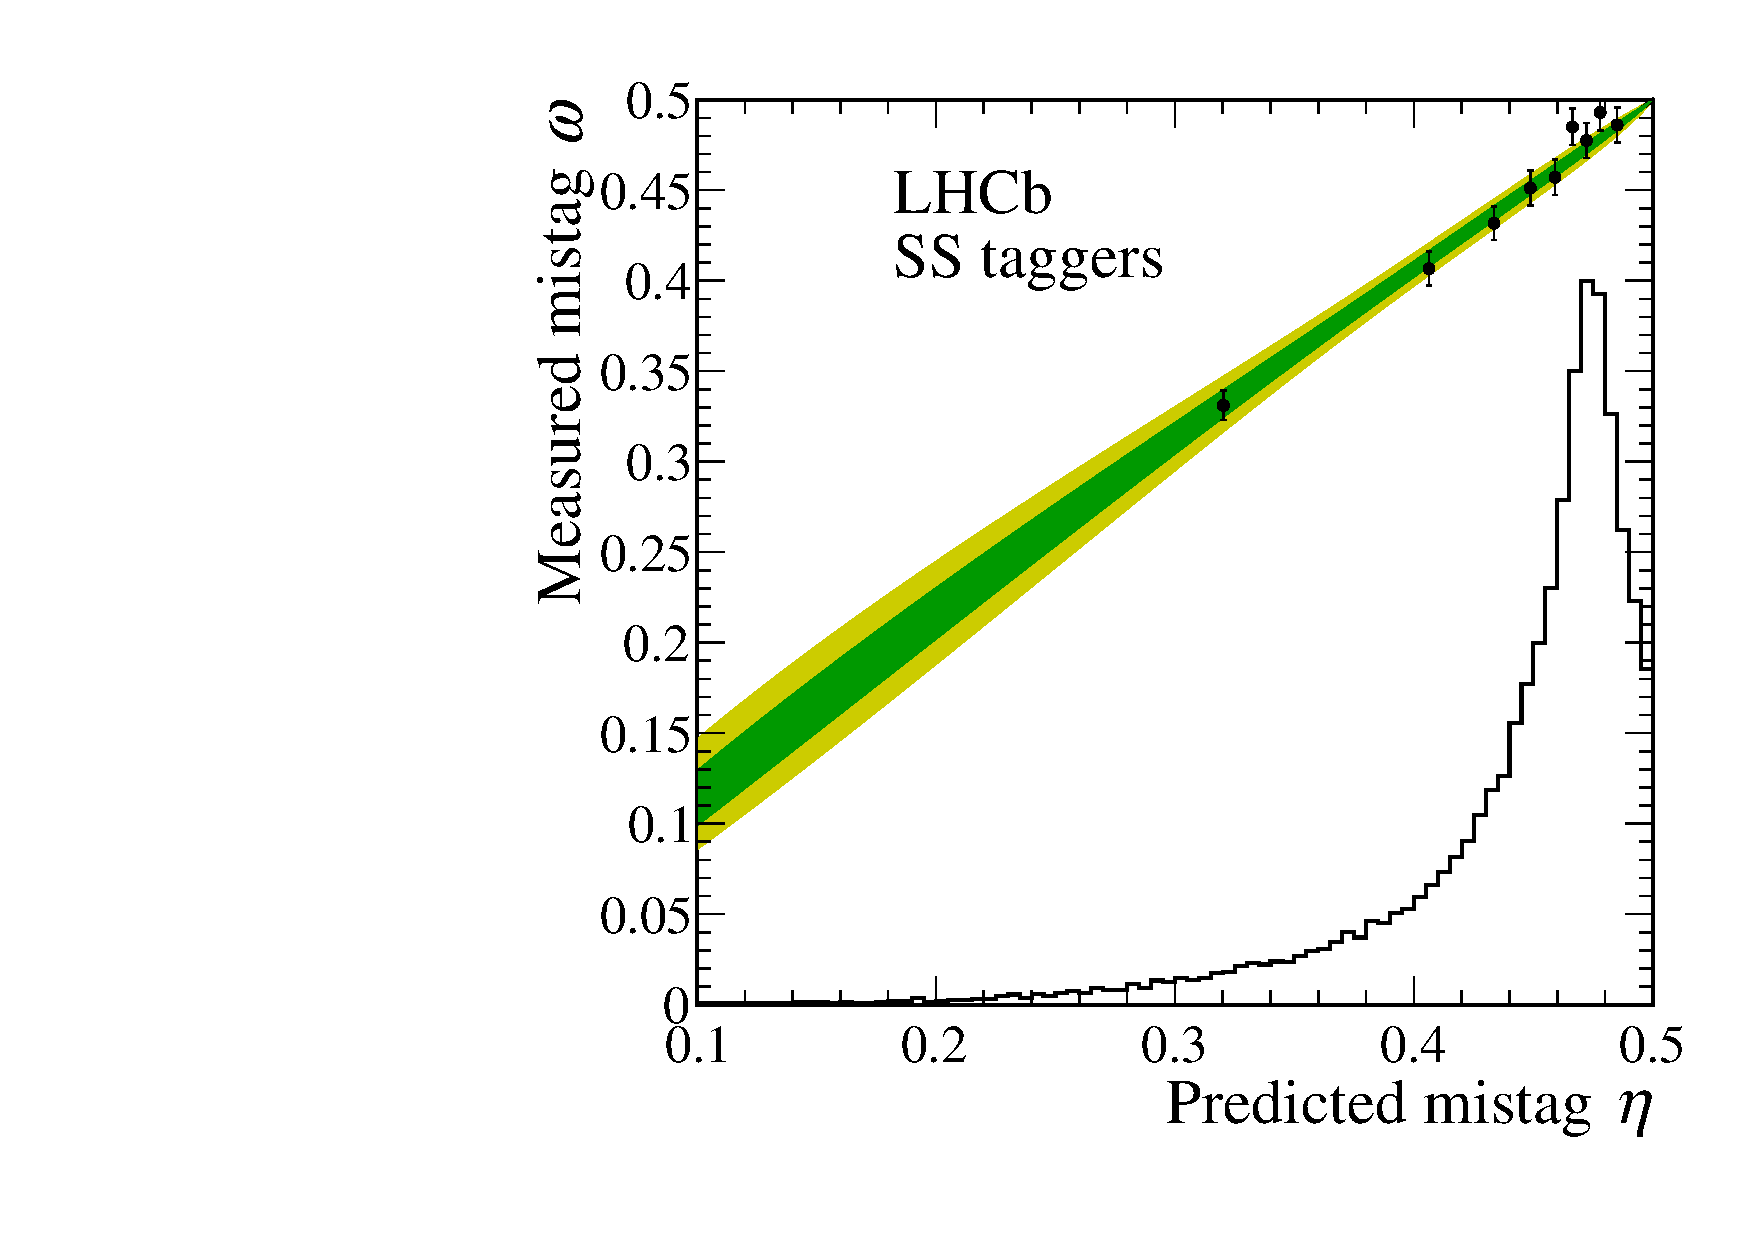
\includegraphics[width=0.45\textwidth]{08FlavourTagging/figs/CalibrationSS.pdf}
	\end{center}
	\caption{Calibration retreived for the SS tagger combination.
	The black histogram is the distributions of the mistag probabilities in arbitrary units.
	The green areas correspond to the \SI{68}{\percent} and \SI{95}{\percent} confidence level regions of the calibration functions.}
	\label{fig:CalibSS}
\end{figure}

The portability of the SS tagger combination is tested on simulated \BdToDpi and $\Bz\!\to\jpsi\Kstarz$ candidates.
This is done using the simulated truth information such that the calibration can be performed in the same way as on a charged decay mode, after equalising the number of initial \Bz- and \Bzb-mesons to separate tagging asymmetries from asymmetries due to \CP-violation or production asymmetries.
Both, the individual calibration parameters and a \enquote{full} comparison from a $\chi^2$ test including the correlations between the parameters, show good agreement (\eg $0.09\sigma$ for the full test).
Despite this good agreement, the parameters in the \CP-fit on \BdToDpi are left free.
On the one hand, this is  motivated by the higher accuracy fo the calibration parameters of the \BdToDpi data sample.
On the other hand this strategy matches the approach for the OS tagger combination, where the portability is not given (\cref{sec:OScalibration}).
In addition, this approach does not require any systematic uncertainty accounting for the portability of the calibration parameters.

\section{Opposite side tagging calibration}
\label{sec:OScalibration}

As mentioned before, the work in this section was done by a collaborator and therefore the explanations will be less detailed than in most other parts of this thesis.

As control channel for the OS tagger combination (namely the OS muon, OS electron, OS kaon, OS vertex charge and OS charm) the charged decay mode $\Bu\!\to\Dz\pip$ is used.
As this decay mode is kinematically  similar to the signal decay \BdToDpi, the same trigger requirements can be applied with a high signal efficiency.
The $\Bu\!\to\Dz\pip$ candidates are further selected by simple rectangular cuts on track quality variables, PID variables, the decay time of the \B-candidate and the invariant mass of the \Dz.
Then a fit to the invariant \Bu mass is performed to extract \emph{sWeights} using the same strategy as in \cref{ch:massfit}.
The invariant mass distribution overlaid with the fit projection from Fit B is shown in \cref{fig:OStaggerMassFit} while \cref{tab:OStaggerMassFitYields} shows the resulting signal and background yields.
\begin{figure}[tbp]
	\begin{center}
		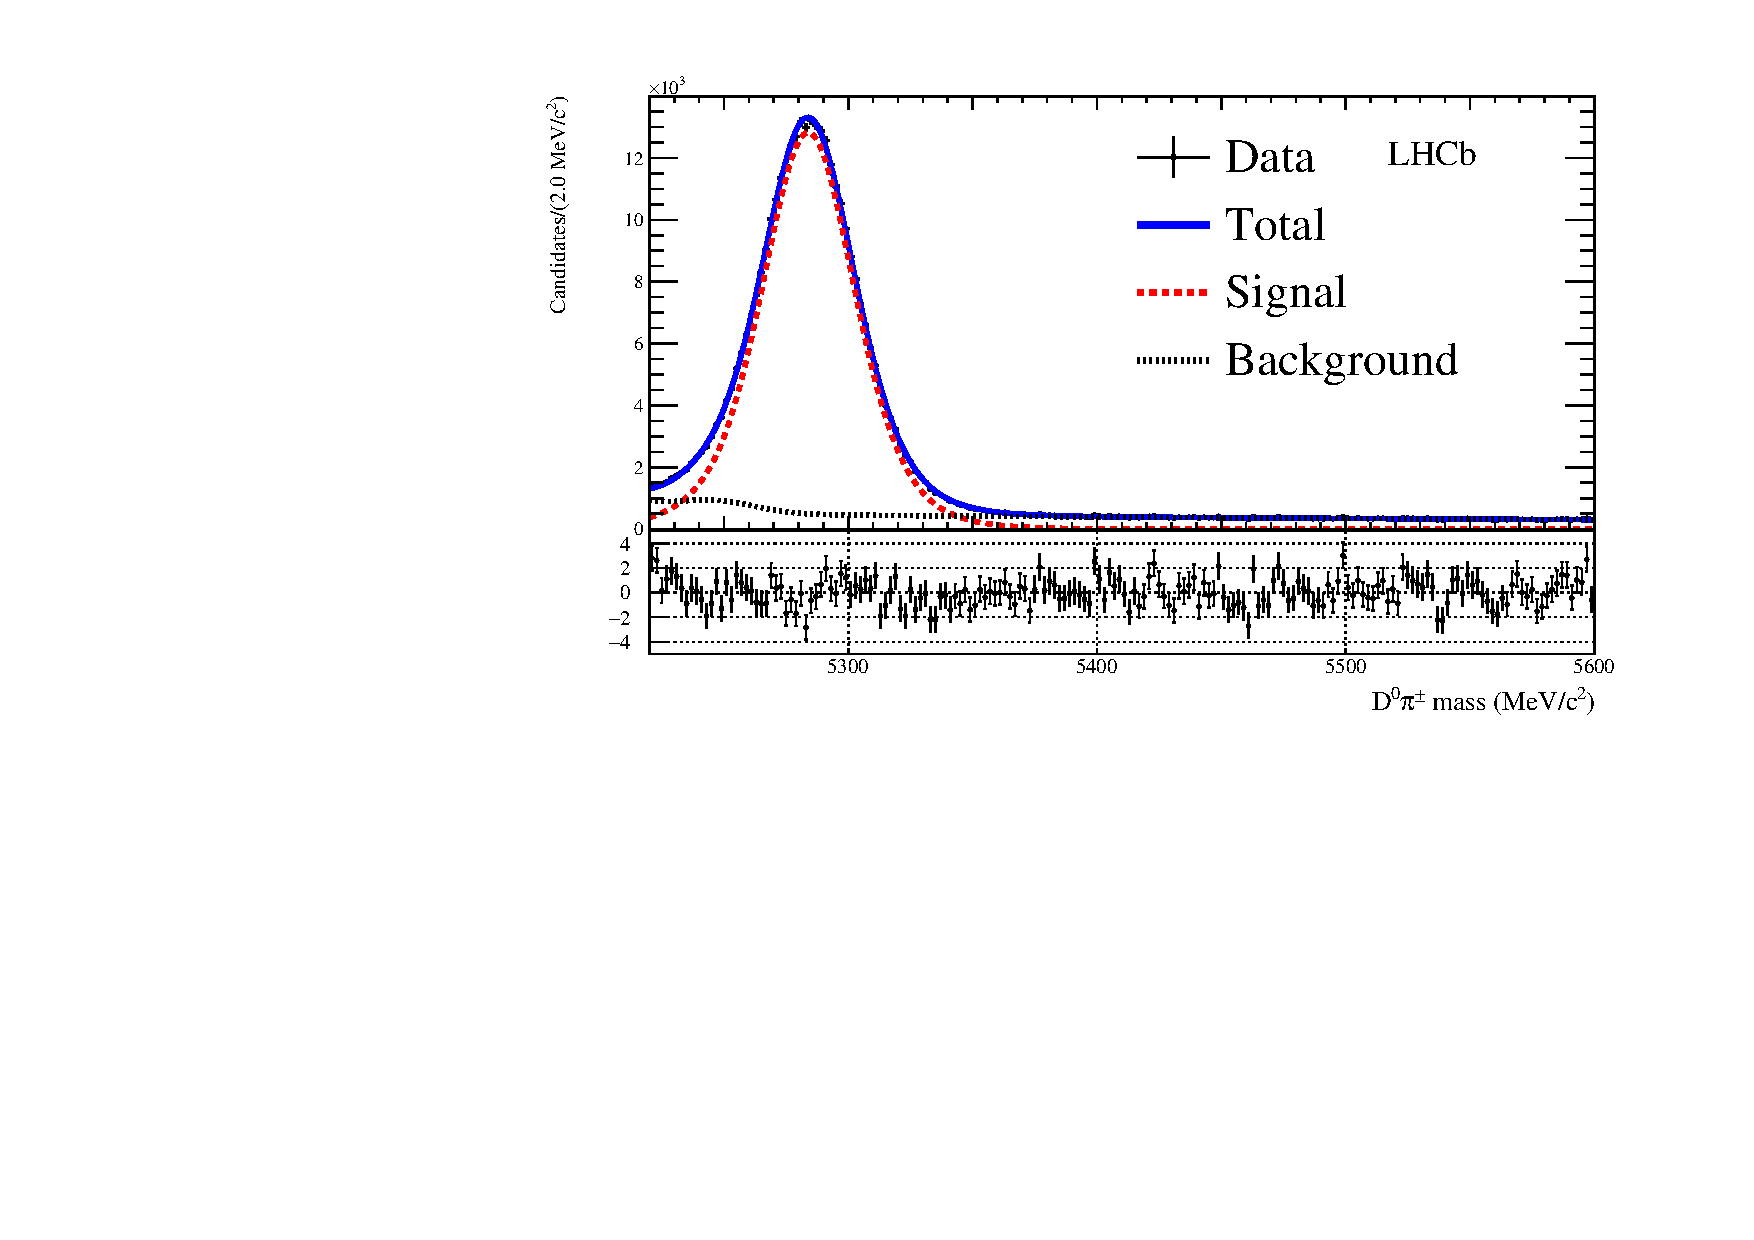
\includegraphics[width=0.7\textwidth]{08FlavourTagging/figs/MDFitForSWeights_BeautyMass_Bu2D0Pi.pdf}
	\end{center}
	\caption{Invariant mass distributions of the $\Dz\pip$ mass.
    The fit projection of Fit B is overlaid.}
	\label{fig:OStaggerMassFit}
\end{figure}
\begin{table}
	\begin{center}
	\caption{Fitted yields of the $\Bu\!\to\Dz\pip$ control channel from Fit B.}
	\begin{tabular}{SS}
		\toprule
		{Parameter} & {Yield} \\
		\midrule
		{$N_{\Bu\!\to\Dz\pip}$}	& 319974\pm612 \\
		{$N_{\text{bkg}}$}		& 85687\pm377 \\
		\bottomrule
	\end{tabular}
	\label{tab:OStaggerMassFitYields}
  \end{center}
\end{table}
Furthermore, the $\Bu\!\to\Dz\pip$ candidates are weighted in the transverse momentum, pseudo-rapidity and decay time of the \B candidate, the number of tracks and PVs in the event and a distribution of trigger decisions to match the distributions of the \BdToDpi candidates.

The calibration model is a GLM with a natural spline function as \emph{basis function} and the modified logistic function from \cref{eq:modlink} as \emph{link function}.
The number of free parameters (\num{10}) in the calibration model is again chosen so that the goodness-of-fit metrics used in \cref{sec:SScombinationcalibration} provide sufficiently satisfactory results.
The comparison with the next simpler model with \num{8} parameters is shown in \cref{tab:GOFOS}.
\begin{table}[tbp]
        \centering
        \caption{GOF metrics for two different calibration models for the OS taggers.}
        \begin{tabular}{SSS}
            \toprule
            {GOF metric} & {Score (8 parameters)} & {Score (10 parameters)} \\
            \midrule
            {$\chi^2$} 	& 4.1312  & -2.197 \\
            {$G^2$} 	& -3.8699 & 0.7199 \\
            $CR$ 		& 2.9273  & -1.6896 \\
            $S$ 		& -4.2701 & 1.8470 \\
            \bottomrule
        \end{tabular}
        \label{tab:GOFOS}
\end{table}
The Calibration is performed using the \emph{sWeights} together with the weights calculated before such that the $\Bu\!\to\Dz\pip$ distributions match the \BdToDpi ones, giving the calibration parameters shown in \cref{tab:CalibOS}.
A graphical representation can be found in \cref{fig:CalibOS}.
\begin{table}[tbp]
	\centering
	\caption{OS calibration parameters obtained on the $\Bu\!\to\Dz\pip$ data sample.}
	\begin{tabular}{ccccc}
		\toprule
		$p_0$ & $p_1$ & $p_2$ & $p_3$ & $p_4$ \\
		\midrule
		\num{-0.136\pm0.019}  & \num{-0.006\pm0.022} & \num{-0.0107\pm0.0083} &\num{-0.45\pm0.10} &\num{-0.85\pm0.46}\\
		\midrule
		$\Delta p_0$ & $\Delta p_1$ & $\Delta p_2$ & $\Delta p_3$ & $\Delta p_4$ \\
		\midrule
		\num{-0.129\pm0.038}  & \num{0.042\pm0.045} & \num{-0.020\pm0.017} &\num{0.42\pm0.21} &\num{1.91\pm0.92}\\
		\bottomrule
	\end{tabular}
	\label{tab:CalibOS}
\end{table}
\begin{figure}[tbp]
	\begin{center}
		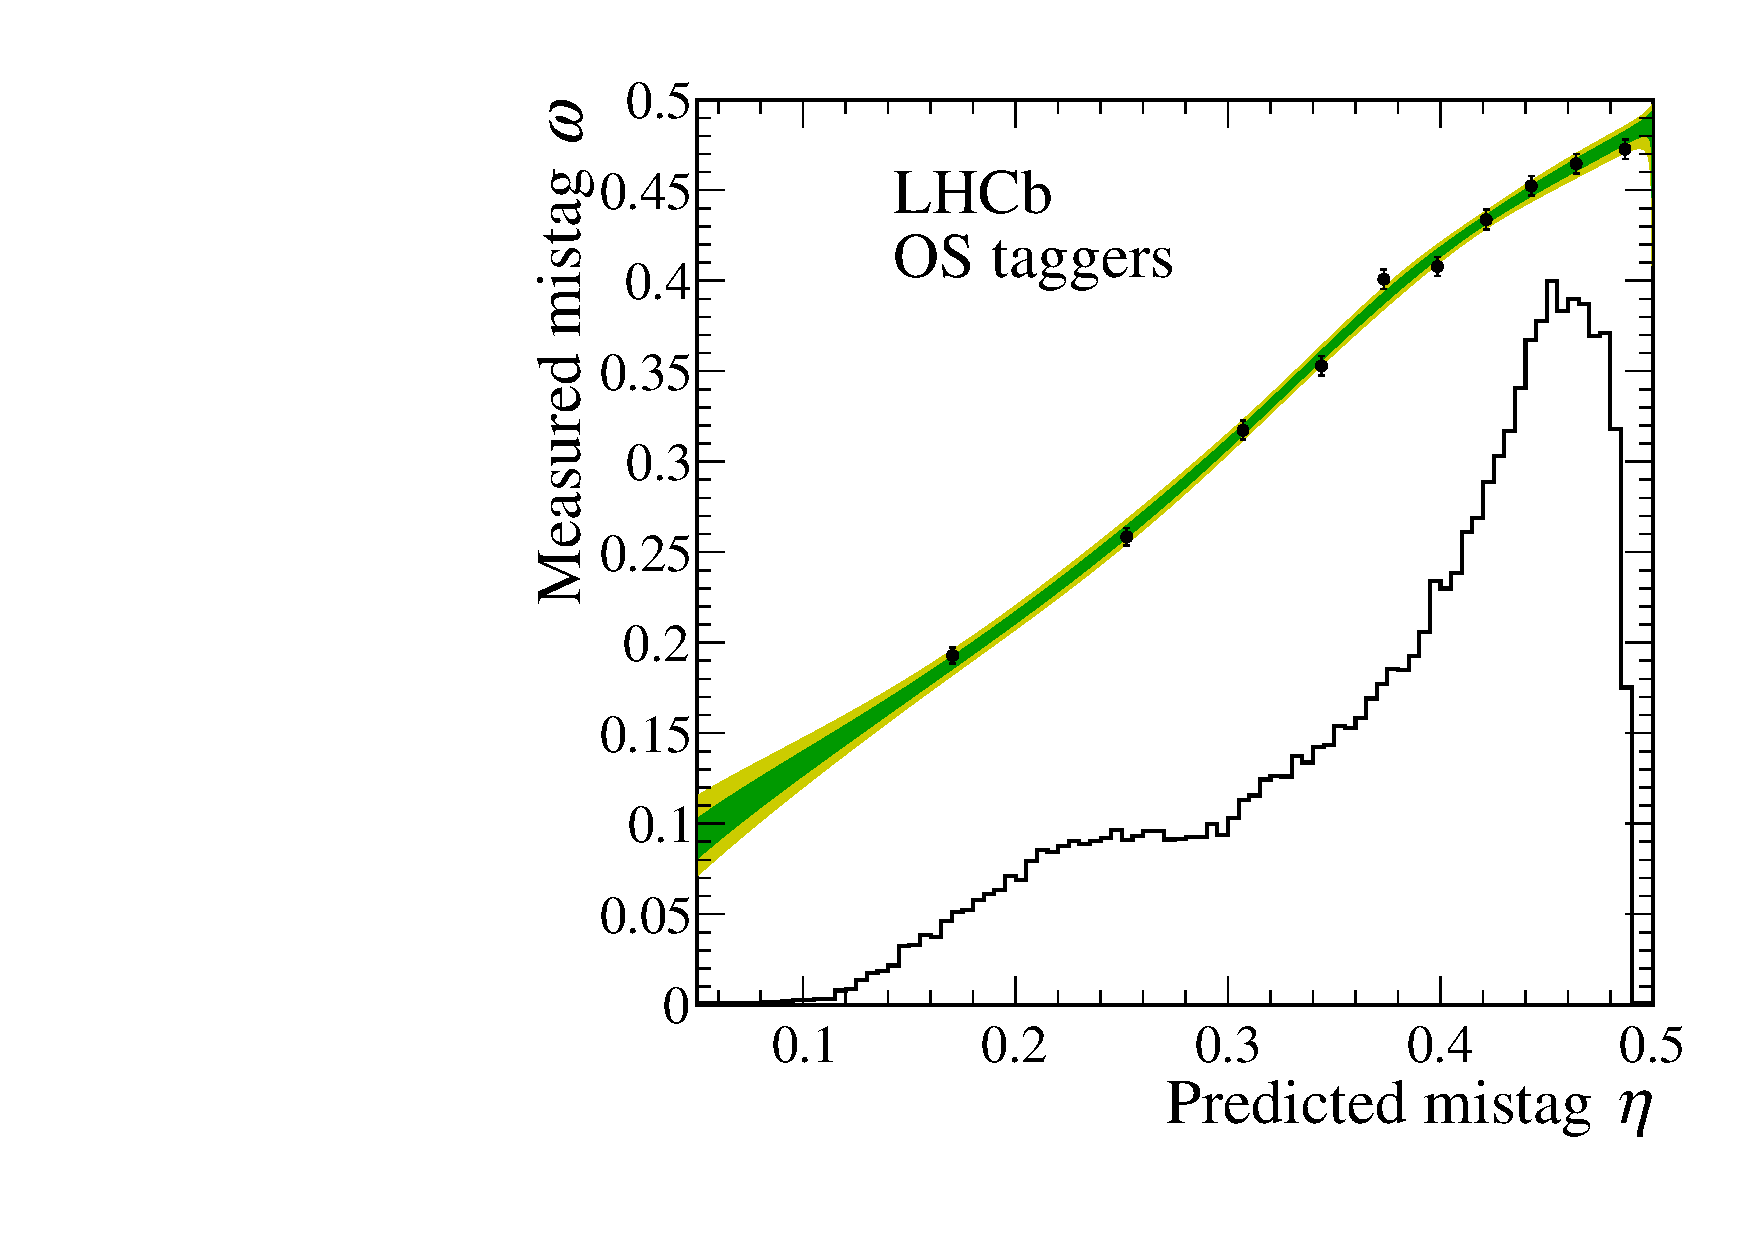
\includegraphics[width=0.45\textwidth]{08FlavourTagging/figs/CalibrationOS.pdf}
	\end{center}
	\caption{Calibration retreived by the for the OS tagger combination.
	The black histogram is the distributions of the mistag probabilities in arbitrary units.
	The shaded areas correspond to the \SI{68}{\percent} and \SI{95}{\percent} confidence level regions of the calibration functions.}
	\label{fig:CalibOS}
\end{figure}

The portability of the calibration is checked on simulated candidates.
The calibration is determined using the simulated true initial flavours on both decay channels after equalising the number of initial \Bz (\Bu) and \Bzb (\Bm) mesons.
The parameters $p_0$ and $p_1$ show deviations of more than $2.5\sigma$, while the full comparison taking into account the correlations between the parameters shows a discrepancy of $2.0\sigma$.
Although one could presume this overall discrepancy is sufficiently small, a study on simulated events presented in \cref{sec:decTimeFitVal} shows that applying the calibration determined on $\Bu\!\to\Dz\pip$ causes a bias for the \CP-parameters \Sf and \Sfbar.
Presumably some residual discrepancies remain despite the weighting of the $\Bu\!\to\Dz\pip$ candidates.
For this reason, the portability is not considered to be given and the calibration is determined directly in the \CP fit on \BdToDpi.
